\PassOptionsToPackage{unicode=true}{hyperref} % options for packages loaded elsewhere
\PassOptionsToPackage{hyphens}{url}
%
\documentclass[11pt,ignorenonframetext,]{beamer}
\usepackage{pgfpages}
\setbeamertemplate{caption}[numbered]
\setbeamertemplate{caption label separator}{: }
\setbeamercolor{caption name}{fg=normal text.fg}
\beamertemplatenavigationsymbolsempty
% Prevent slide breaks in the middle of a paragraph:
\widowpenalties 1 10000
\raggedbottom
\setbeamertemplate{part page}{
\centering
\begin{beamercolorbox}[sep=16pt,center]{part title}
  \usebeamerfont{part title}\insertpart\par
\end{beamercolorbox}
}
\setbeamertemplate{section page}{
\centering
\begin{beamercolorbox}[sep=12pt,center]{part title}
  \usebeamerfont{section title}\insertsection\par
\end{beamercolorbox}
}
\setbeamertemplate{subsection page}{
\centering
\begin{beamercolorbox}[sep=8pt,center]{part title}
  \usebeamerfont{subsection title}\insertsubsection\par
\end{beamercolorbox}
}
\AtBeginPart{
  \frame{\partpage}
}
\AtBeginSection{
  \ifbibliography
  \else
    \frame{\sectionpage}
  \fi
}
\AtBeginSubsection{
  \frame{\subsectionpage}
}
\usepackage{lmodern}
\usepackage{amssymb,amsmath}
\usepackage{ifxetex,ifluatex}
\usepackage{fixltx2e} % provides \textsubscript
\ifnum 0\ifxetex 1\fi\ifluatex 1\fi=0 % if pdftex
  \usepackage[T1]{fontenc}
  \usepackage[utf8]{inputenc}
  \usepackage{textcomp} % provides euro and other symbols
\else % if luatex or xelatex
  \usepackage{unicode-math}
  \defaultfontfeatures{Ligatures=TeX,Scale=MatchLowercase}
\fi
\usetheme[]{metropolis}
% use upquote if available, for straight quotes in verbatim environments
\IfFileExists{upquote.sty}{\usepackage{upquote}}{}
% use microtype if available
\IfFileExists{microtype.sty}{%
\usepackage[]{microtype}
\UseMicrotypeSet[protrusion]{basicmath} % disable protrusion for tt fonts
}{}
\IfFileExists{parskip.sty}{%
\usepackage{parskip}
}{% else
\setlength{\parindent}{0pt}
\setlength{\parskip}{6pt plus 2pt minus 1pt}
}
\usepackage{hyperref}
\hypersetup{
            pdftitle={Lecture 9},
            pdfborder={0 0 0},
            breaklinks=true}
\urlstyle{same}  % don't use monospace font for urls
\newif\ifbibliography
\usepackage{color}
\usepackage{fancyvrb}
\newcommand{\VerbBar}{|}
\newcommand{\VERB}{\Verb[commandchars=\\\{\}]}
\DefineVerbatimEnvironment{Highlighting}{Verbatim}{commandchars=\\\{\}}
% Add ',fontsize=\small' for more characters per line
\newenvironment{Shaded}{}{}
\newcommand{\AlertTok}[1]{\textcolor[rgb]{1.00,0.00,0.00}{\textbf{#1}}}
\newcommand{\AnnotationTok}[1]{\textcolor[rgb]{0.38,0.63,0.69}{\textbf{\textit{#1}}}}
\newcommand{\AttributeTok}[1]{\textcolor[rgb]{0.49,0.56,0.16}{#1}}
\newcommand{\BaseNTok}[1]{\textcolor[rgb]{0.25,0.63,0.44}{#1}}
\newcommand{\BuiltInTok}[1]{#1}
\newcommand{\CharTok}[1]{\textcolor[rgb]{0.25,0.44,0.63}{#1}}
\newcommand{\CommentTok}[1]{\textcolor[rgb]{0.38,0.63,0.69}{\textit{#1}}}
\newcommand{\CommentVarTok}[1]{\textcolor[rgb]{0.38,0.63,0.69}{\textbf{\textit{#1}}}}
\newcommand{\ConstantTok}[1]{\textcolor[rgb]{0.53,0.00,0.00}{#1}}
\newcommand{\ControlFlowTok}[1]{\textcolor[rgb]{0.00,0.44,0.13}{\textbf{#1}}}
\newcommand{\DataTypeTok}[1]{\textcolor[rgb]{0.56,0.13,0.00}{#1}}
\newcommand{\DecValTok}[1]{\textcolor[rgb]{0.25,0.63,0.44}{#1}}
\newcommand{\DocumentationTok}[1]{\textcolor[rgb]{0.73,0.13,0.13}{\textit{#1}}}
\newcommand{\ErrorTok}[1]{\textcolor[rgb]{1.00,0.00,0.00}{\textbf{#1}}}
\newcommand{\ExtensionTok}[1]{#1}
\newcommand{\FloatTok}[1]{\textcolor[rgb]{0.25,0.63,0.44}{#1}}
\newcommand{\FunctionTok}[1]{\textcolor[rgb]{0.02,0.16,0.49}{#1}}
\newcommand{\ImportTok}[1]{#1}
\newcommand{\InformationTok}[1]{\textcolor[rgb]{0.38,0.63,0.69}{\textbf{\textit{#1}}}}
\newcommand{\KeywordTok}[1]{\textcolor[rgb]{0.00,0.44,0.13}{\textbf{#1}}}
\newcommand{\NormalTok}[1]{#1}
\newcommand{\OperatorTok}[1]{\textcolor[rgb]{0.40,0.40,0.40}{#1}}
\newcommand{\OtherTok}[1]{\textcolor[rgb]{0.00,0.44,0.13}{#1}}
\newcommand{\PreprocessorTok}[1]{\textcolor[rgb]{0.74,0.48,0.00}{#1}}
\newcommand{\RegionMarkerTok}[1]{#1}
\newcommand{\SpecialCharTok}[1]{\textcolor[rgb]{0.25,0.44,0.63}{#1}}
\newcommand{\SpecialStringTok}[1]{\textcolor[rgb]{0.73,0.40,0.53}{#1}}
\newcommand{\StringTok}[1]{\textcolor[rgb]{0.25,0.44,0.63}{#1}}
\newcommand{\VariableTok}[1]{\textcolor[rgb]{0.10,0.09,0.49}{#1}}
\newcommand{\VerbatimStringTok}[1]{\textcolor[rgb]{0.25,0.44,0.63}{#1}}
\newcommand{\WarningTok}[1]{\textcolor[rgb]{0.38,0.63,0.69}{\textbf{\textit{#1}}}}
\usepackage{longtable,booktabs}
\usepackage{caption}
% These lines are needed to make table captions work with longtable:
\makeatletter
\def\fnum@table{\tablename~\thetable}
\makeatother
\setlength{\emergencystretch}{3em}  % prevent overfull lines
\providecommand{\tightlist}{%
  \setlength{\itemsep}{0pt}\setlength{\parskip}{0pt}}
\setcounter{secnumdepth}{0}

% set default figure placement to htbp
\makeatletter
\def\fps@figure{htbp}
\makeatother

\usepackage{geometry}
\usepackage{graphicx}

\usepackage{bbold}
\usepackage{lmodern}


\usepackage{url}		% produces hyperlinks

\usepackage{colortbl}	% allows for color usage in tables
\usepackage{multirow}	% allows for rows that span multiple rows in tables

\usepackage{color}          	% gives color options
\usepackage{xcolor}		% this package has a variety of color options

\usepackage{multicol}
\usepackage{textcomp}

\usepackage{setspace}
\usepackage{changepage}
\usepackage{isotope}

\singlespacing

\def\begincol{\begin{column}}
\def\endcol{\end{column}}

\def\begincols{\begin{columns}}
\def\endcols{\end{columns}}

%%%%%%%%%%%%%%%%
% Small code output
%%%%%%%%%%%%%%%%

%% change fontsize of R code

\makeatletter
\@ifundefined{Shaded}{\newenvironment{Shaded}{}{}}{}
\makeatother


\let\oldShaded\Shaded
\let\endoldShaded\endShaded
\renewenvironment{Shaded}{\footnotesize\begin{spacing}{0.9}\oldShaded}{\endoldShaded\end{spacing}}

%% change fontsize of output
\let\oldverbatim\verbatim
\let\endoldverbatim\endverbatim
\renewenvironment{verbatim}{\footnotesize\begin{spacing}{0.9}\oldverbatim}{\endoldverbatim\end{spacing}}


\newcommand{\tinyoutput}{
  \renewenvironment{Shaded}{\tiny\begin{spacing}{0.9}\oldShaded}{\endoldShaded\end{spacing}}
  \renewenvironment{verbatim}{\tiny\begin{spacing}{0.9}\oldverbatim}{\endoldverbatim\end{spacing}}
}

\newcommand{\scriptoutput}{
  \renewenvironment{Shaded}{\scriptsize\begin{spacing}{0.9}\oldShaded}{\endoldShaded\end{spacing}}
  \renewenvironment{verbatim}{\scriptsize\begin{spacing}{0.9}\oldverbatim}{\endoldverbatim\end{spacing}}
}

\newcommand{\footnoteoutput}{
  \renewenvironment{Shaded}{\footnotesize\begin{spacing}{0.9}\oldShaded}{\endoldShaded\end{spacing}}
  \renewenvironment{verbatim}{\footnotesize\begin{spacing}{0.9}\oldverbatim}{\endoldverbatim\end{spacing}}
}

%\newcommand{\verbatimfont}[1]{\renewcommand{\verbatim@font}{\ttfamily#1}}


%%%%%%%%%%%%%%%%
% Custom Colors
%%%%%%%%%%%%%%%%

\definecolor{redhl}{rgb}{0.98,0.29,0.28}
\definecolor{yellowhl}{rgb}{0.98,0.87,0.28}


\xdefinecolor{oiBlue}{rgb}{0.15, 0.35, 0.55}
\xdefinecolor{gray}{rgb}{0.5, 0.5, 0.5}
\xdefinecolor{darkGray}{rgb}{0.3, 0.3, 0.3}
\xdefinecolor{darkerGray}{rgb}{0.2, 0.2, 0.2}
\xdefinecolor{rubineRed}{rgb}{0.89,0,0.30}
\xdefinecolor{linkCol}{rgb}{0.11,0.49,0.95}	
\xdefinecolor{irishGreen}{rgb}{0,0.60,0}	
\xdefinecolor{darkturquoise}{rgb}{0.44, 0.58, 0.86}
\definecolor{lightGreen}{rgb}{0.533,0.765,0.42}
%\xdefinecolor{hlblue}{rgb}{0.051,0.65,1}
\xdefinecolor{hlblue}{rgb}{ 0.055, 0.639, 0.831}
\definecolor{light}{rgb}{.337,.608,.741}
\definecolor{dark}{rgb}{.337,.608,.741}

\definecolor{cpink}{rgb}{0.93, 0.23, 0.51}

%%%%%%%%%%%%%%%%
% Custom Commands
%%%%%%%%%%%%%%%%

% text colors
\newcommand{\red}[1]{\textit{\textcolor{rubineRed}{#1}}}
\newcommand{\orange}[1]{\textit{\textcolor{orange}{#1}}}
\newcommand{\pink}[1]{\textit{\textcolor{rubineRed!90!white!50}{#1}}}
\newcommand{\green}[1]{\textit{\textcolor{irishGreen}{#1}}}
\newcommand{\blue}[1]{\textit{\textcolor{darkturquoise}{#1}}}
\newcommand{\light}[1]{\textcolor{light}{\textbf{#1}}}
\newcommand{\dark}[1]{\textcolor{dark}{#1}}
\newcommand{\gray}[1]{\textcolor{gray}{#1}}


% mail
\newcommand{\mail}[1]{\href{mailto:#1}{\textit{\textcolor{linkCol}{#1}}}}

% highlighting: hl, hlGr, mathhl
\newcommand{\hl}[1]{\textit{\textcolor{hlblue}{#1}}}
\newcommand{\hlGr}[1]{\textit{\textcolor{lightGreen}{#1}}}
\newcommand{\hlRd}[1]{\textit{\textcolor{rubineRed}{#1}}}
\newcommand{\mathhl}[1]{\textcolor{hlblue}{\ensuremath{#1}}}
\newcommand{\hlr}[1]{\fcolorbox{redhl}{white}{$\displaystyle #1$}}
\newcommand{\hly}[1]{\fcolorbox{yellowhl}{white}{$\displaystyle #1$}}


\newcommand{\vvfill}{\vskip0pt plus 1filll}

\DeclareMathOperator*{\argmin}{arg\,min}
\DeclareMathOperator*{\argmax}{arg\,max}

\title{Lecture 9}
\providecommand{\subtitle}[1]{}
\subtitle{ARIMA Models}
\date{10/03/2018}

\begin{document}
\frame{\titlepage}

\hypertarget{mainfty}{%
\section{\texorpdfstring{\(MA(\infty)\)}{MA(\textbackslash{}infty)}}\label{mainfty}}

\begin{frame}[t]{\(MA(q)\)}
\protect\hypertarget{maq}{}

From last time,
\[ MA(q): \qquad y_t = \delta + w_t + \theta_1 \, w_{t-1} + \theta_2 \, w_{t-2} + \cdots + \theta_q \, w_{t-q} \]

Properties: \[E(y_t) = \delta\]

\[
\gamma(0) = Var(y_t) = (1 + \theta_1^2 + \theta_2 + \cdots + \theta_q^2) \, \sigma_w^2
\]

\[
\gamma(h) = 
\begin{cases}
\theta_h + \theta_1 \, \theta_{1+h} + \theta_2 \, \theta_{2+h} + \cdots + \theta_{q-h}\, \theta_{q} & \text{if } h\in\{1,\ldots,q\} \\
0 & \text{otherwise}
\end{cases}
\]

and is stationary for any values of \((\theta_1, \ldots,\theta_q)\)

\end{frame}

\begin{frame}[t]{\(MA(\infty)\)}
\protect\hypertarget{mainfty-1}{}

If we let \(q \to \infty\) then process will be stationary if and only
if the moving average coefficients (\(\theta\) 's) are square summable,
i.e.

\[ \sum_{i=1}^\infty \theta_i^2 < \infty \]

which is necessary such that \(Var(y_t) < \infty\) so that the weak
stationarity are met.

\(~\)

Sometimes, a slightly stronger condition known as absolute summability,
\[\sum_{i=1}^\infty |\theta_i| < \infty\], is necessary (e.g.~for some
CLT related asymptotic results).

\end{frame}

\begin{frame}[t]{Invertibility}
\protect\hypertarget{invertibility}{}

If an \(MA(q)\) process, \(y_t = \delta + \theta_q(L) w_t\), can be
rewritten as a stationary \(AR\) process then the process is said to be
invertible.

\(MA(1)\) w/ \(\delta=0\) example:

\end{frame}

\begin{frame}[t]{Invertibility vs Stationarity}
\protect\hypertarget{invertibility-vs-stationarity}{}

A \(MA(q)\) process is \emph{invertible} if
\(y_t = \delta + \theta_q(L) \, w_t\) can be rewritten as an exclusively
\(AR\) process (of possibly infinite order), i.e.
\(\phi(L) \, y_t = \alpha + w_t\).

\(~\)

\pause

Conversely, an \(AR(p)\) process is \emph{stationary} if
\(\phi_p(L) \, y_t = \delta + w_t\) can be rewritten as an exclusively
\(MA\) process (of possibly infinite order), i.e.
\(y_t = \delta + \theta(L) \, w_t\).

\(~\)

\pause

So using our results w.r.t. \(\phi(L)\) it follows that if all of the
roots of \(\theta_q(L)\) are outside the complex unit circle then the
moving average process is invertible.

\end{frame}

\hypertarget{differencing}{%
\section{Differencing}\label{differencing}}

\begin{frame}{Difference operator}
\protect\hypertarget{difference-operator}{}

We will need to define one more notational tool for indicating
differencing \[ \Delta y_t = y_t - y_{t-1} \]

\pause

Just like the lag operator we will indicate repeated applications of
this operator using exponents \[ 
\begin{aligned}
\Delta^2 y_t 
  &= \Delta (\Delta y_t) \\
  &= (\Delta y_t) - (\Delta y_{t-1}) \\
  &= (y_t - y_{t-1}) - (y_{t-1} - y_{t-2}) \\
  &= y_t - 2y_{t-1}+y_{t-2}
\end{aligned}
\]

\pause

Note that \(\Delta\) can even be expressed in terms of the lag operator
\(L\), \[ \Delta^d = (1-L)^d \]

\end{frame}

\begin{frame}[t]{Differencing and Stocastic Trend}
\protect\hypertarget{differencing-and-stocastic-trend}{}

Using the two component time series model \[ y_t = \mu_t + x_t \] where
\(\mu_t\) is a non-stationary trend component and \(x_t\) is a mean zero
stationary component.

\(~\)

We have already shown that differencing can address deterministic trend
(e.g. \(\mu_t = \beta_0+\beta_1 \, t\)). In fact, if \(\mu_t\) is any
\(k\)-th order polynomial of \(t\) then \(\Delta^k y_t\) is stationary.

\(~\)

Differencing can also address stochastic trend such as in the case where
\(\mu_t\) follows a random walk.

\end{frame}

\begin{frame}[t]{Stochastic trend - Example 1}
\protect\hypertarget{stochastic-trend---example-1}{}

Let \(y_t = \mu_t + w_t\) where \(w_t\) is white noise and
\(\mu_t = \mu_{t-1} + v_t\) with \(v_t\) being a stationary process with
mean 0.

\begin{center}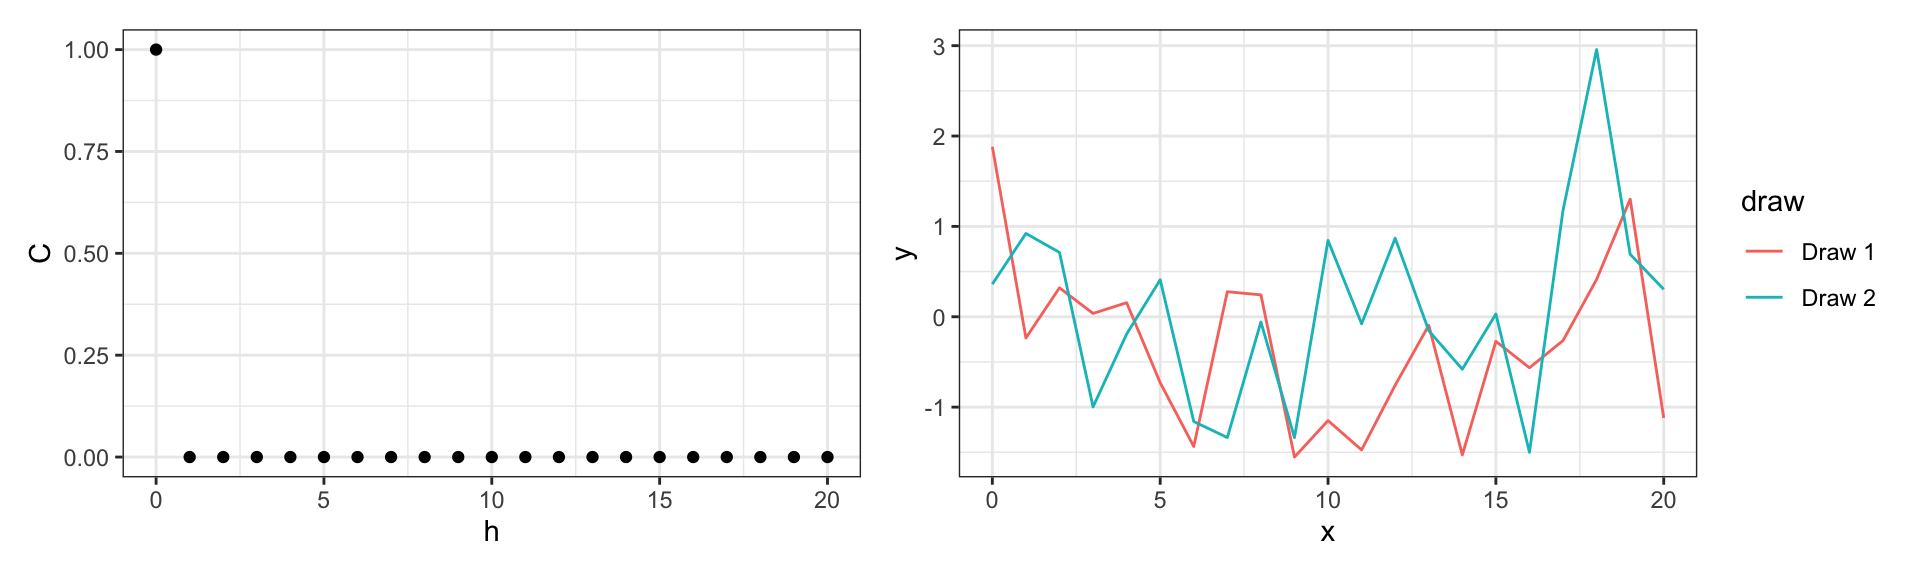
\includegraphics[width=\textwidth]{Lec09_files/figure-beamer/unnamed-chunk-1-1} \end{center}

\end{frame}

\begin{frame}[fragile]{Differenced stochastic trend}
\protect\hypertarget{differenced-stochastic-trend}{}

\begin{Shaded}
\begin{Highlighting}[]
\NormalTok{forecast}\OperatorTok{::}\KeywordTok{ggtsdisplay}\NormalTok{(}\KeywordTok{diff}\NormalTok{(d}\OperatorTok{$}\NormalTok{y))}
\end{Highlighting}
\end{Shaded}

\begin{center}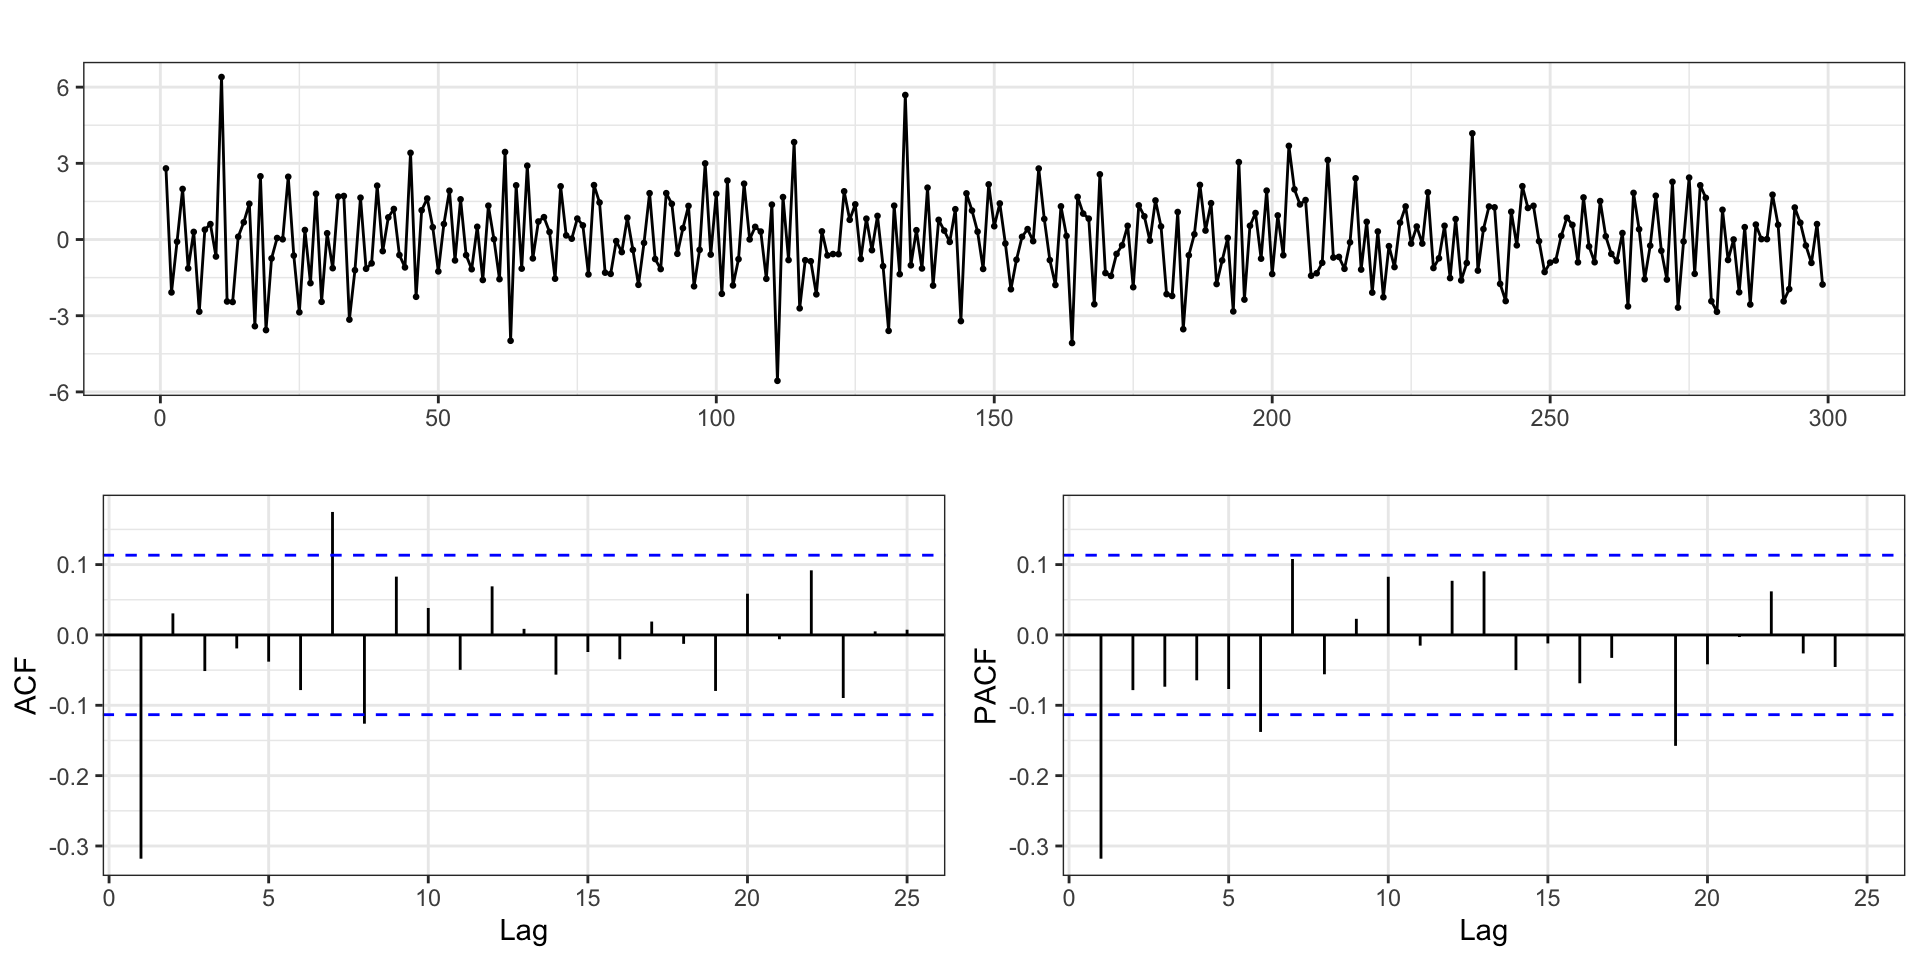
\includegraphics[width=\textwidth]{Lec09_files/figure-beamer/unnamed-chunk-2-1} \end{center}

\end{frame}

\begin{frame}[t]{Stationary?}
\protect\hypertarget{stationary}{}

Is \(y_t\) stationary?

\end{frame}

\begin{frame}[t]{Difference Stationary?}
\protect\hypertarget{difference-stationary}{}

Is \(\Delta y_t\) stationary?

\end{frame}

\begin{frame}[t]{Stochastic trend - Example 2}
\protect\hypertarget{stochastic-trend---example-2}{}

Let \(y_t = \mu_t + w_t\) where \(w_t\) is white noise and
\(\mu_t = \mu_{t-1} + v_t\) but now \(v_t = v_{t-1} + e_t\) with \(e_t\)
being stationary.

\begin{center}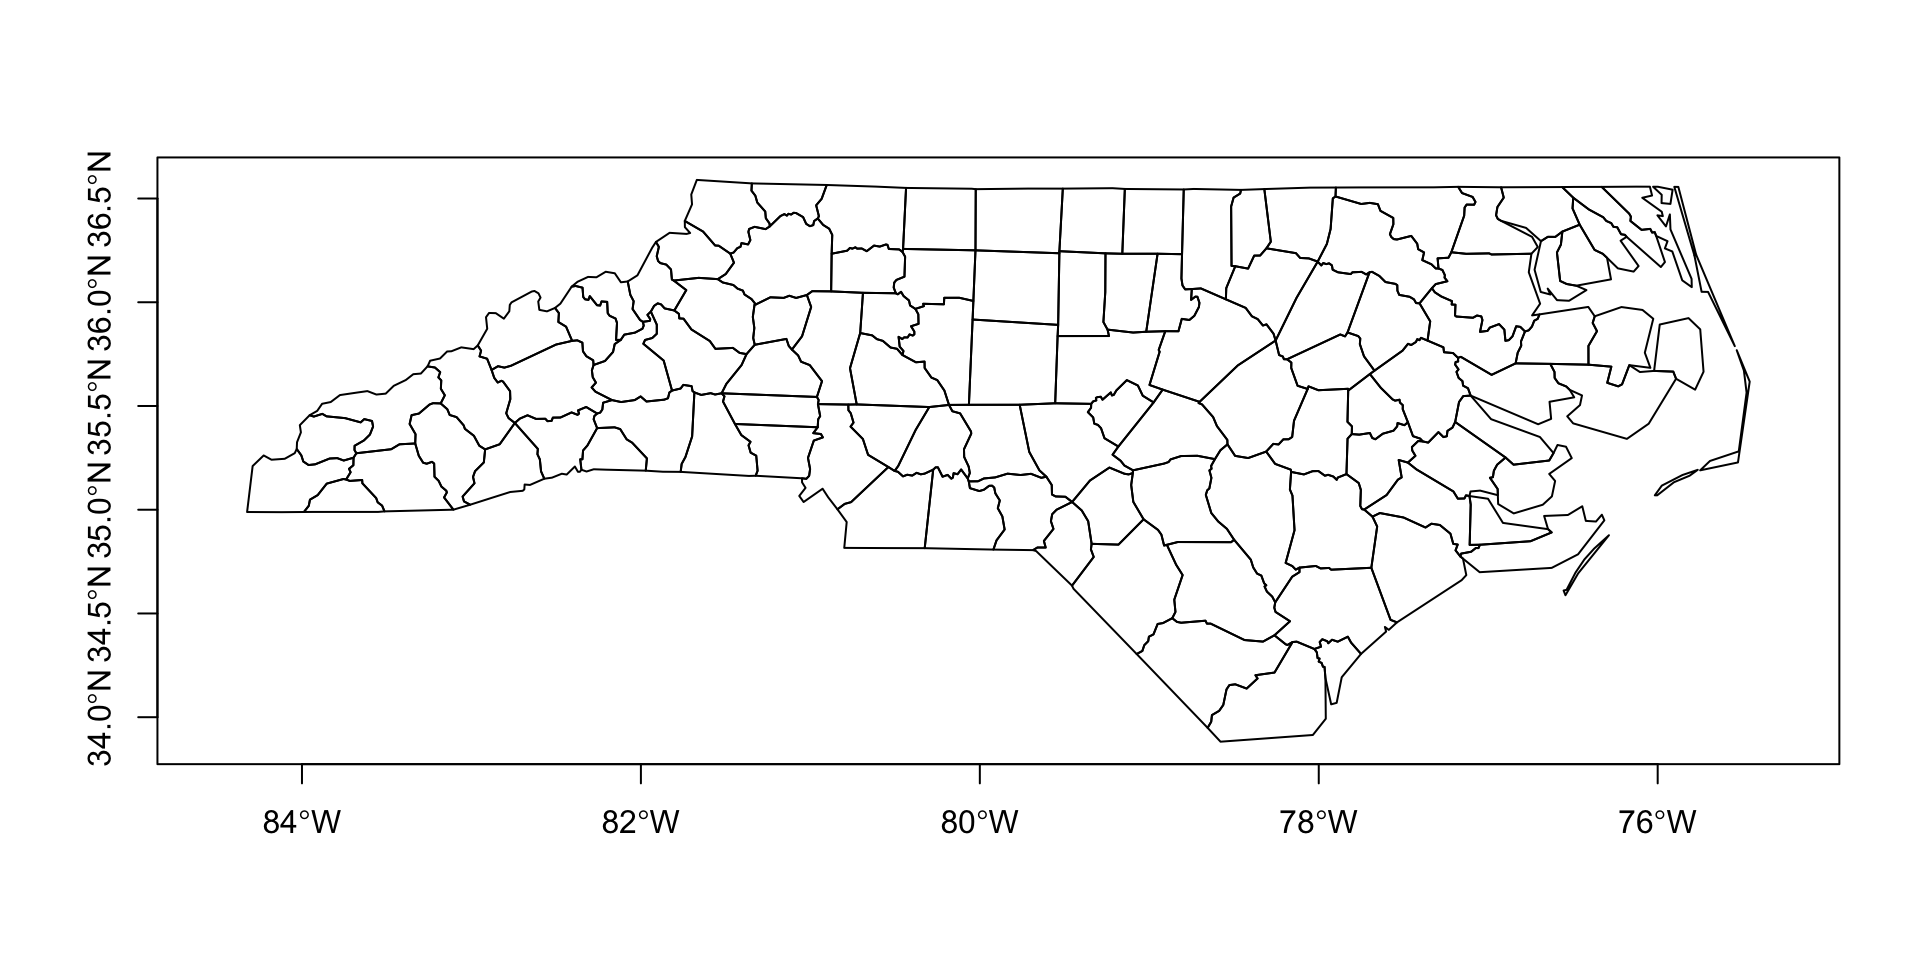
\includegraphics[width=\textwidth]{Lec09_files/figure-beamer/unnamed-chunk-3-1} \end{center}

\end{frame}

\begin{frame}[fragile]{Differenced stochastic trend}
\protect\hypertarget{differenced-stochastic-trend-1}{}

\begin{Shaded}
\begin{Highlighting}[]
\NormalTok{forecast}\OperatorTok{::}\KeywordTok{ggtsdisplay}\NormalTok{(}\KeywordTok{diff}\NormalTok{(d}\OperatorTok{$}\NormalTok{y))}
\end{Highlighting}
\end{Shaded}

\begin{center}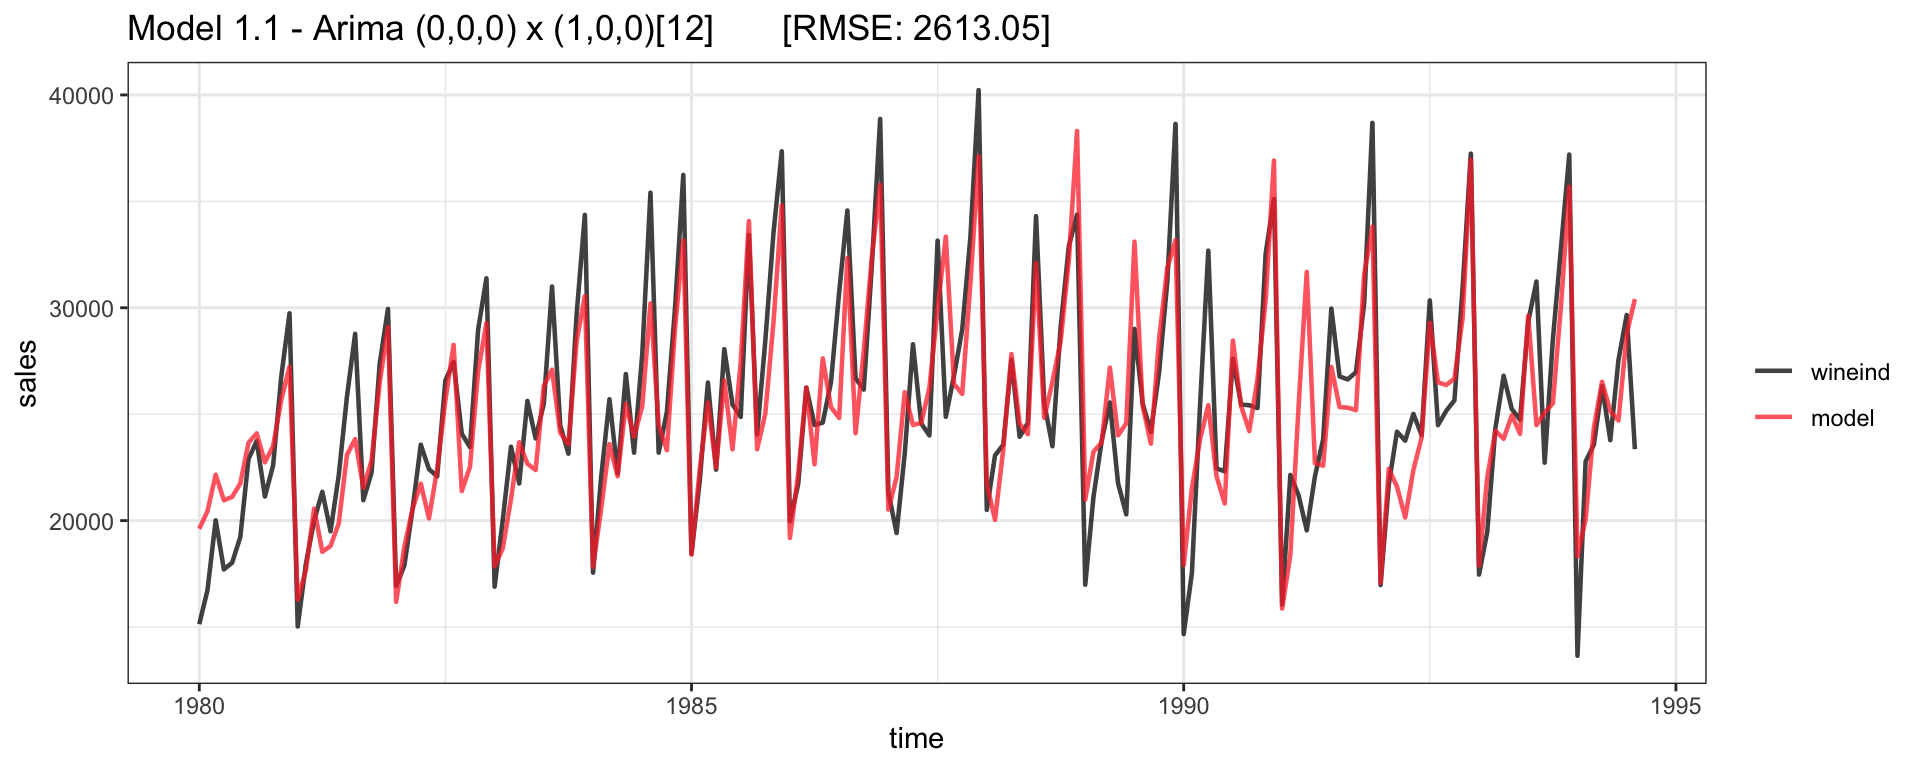
\includegraphics[width=\textwidth]{Lec09_files/figure-beamer/unnamed-chunk-4-1} \end{center}

\end{frame}

\begin{frame}[fragile]{Twice differenced stochastic trend}
\protect\hypertarget{twice-differenced-stochastic-trend}{}

\begin{Shaded}
\begin{Highlighting}[]
\NormalTok{forecast}\OperatorTok{::}\KeywordTok{ggtsdisplay}\NormalTok{(}\KeywordTok{diff}\NormalTok{(d}\OperatorTok{$}\NormalTok{y,}\DataTypeTok{differences =} \DecValTok{2}\NormalTok{))}
\end{Highlighting}
\end{Shaded}

\begin{center}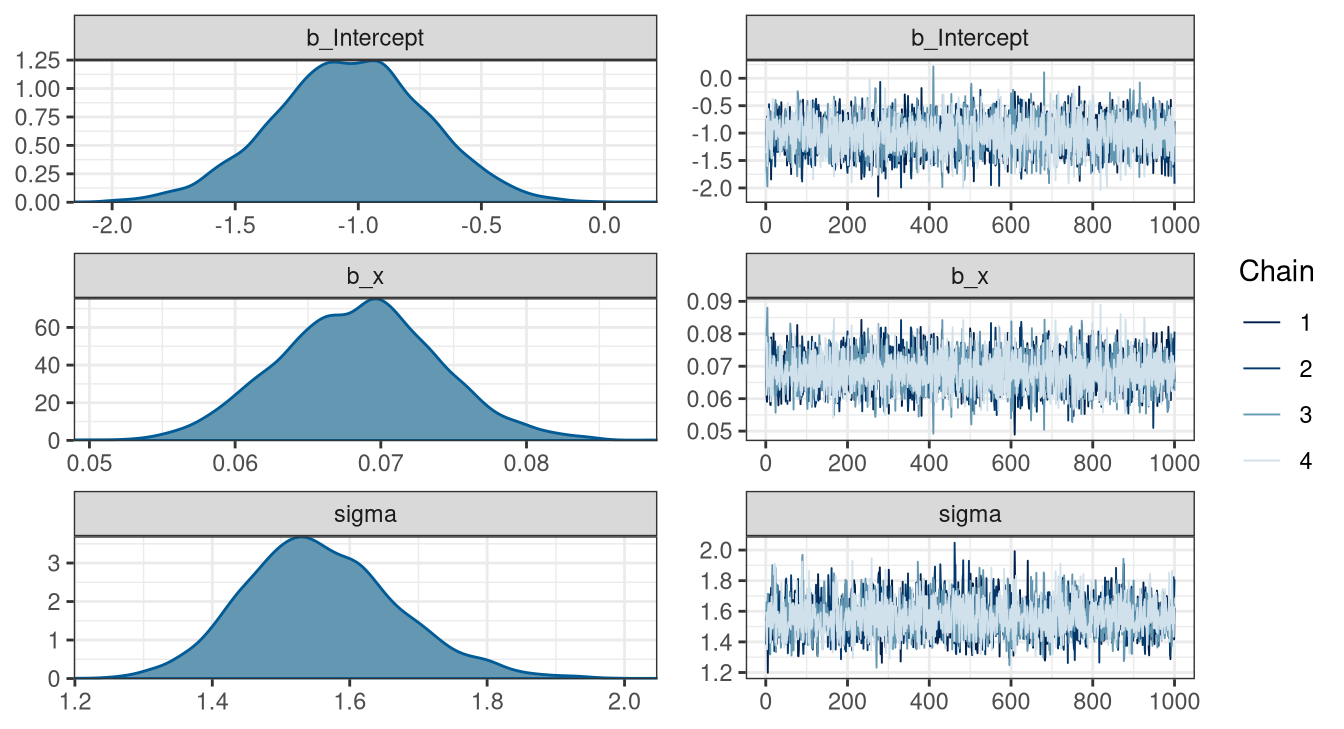
\includegraphics[width=\textwidth]{Lec09_files/figure-beamer/unnamed-chunk-5-1} \end{center}

\end{frame}

\begin{frame}[t]{Difference stationary?}
\protect\hypertarget{difference-stationary-1}{}

Is \(\Delta y_t\) stationary?

\end{frame}

\begin{frame}[t]{2nd order difference stationary?}
\protect\hypertarget{nd-order-difference-stationary}{}

What about \(\Delta^2 y_t\), is it stationary?

\end{frame}

\hypertarget{arima}{%
\section{\texorpdfstring{\(ARIMA\)}{ARIMA}}\label{arima}}

\begin{frame}{\(ARIMA\) Models}
\protect\hypertarget{arima-models}{}

Autoregressive integrated moving average are just an extension of an
\(ARMA\) model to include differencing of degree \(d\) to \(y_t\) before
including the autoregressive and moving average components.

\[
\begin{aligned}
ARIMA(p,d,q): \qquad \phi_p(L) \; \Delta^d \, y_t &= \delta + \theta_q(L) w_t  
\end{aligned}
\]

\pause

\(~\)

Box-Jenkins approach:

\begin{enumerate}
\item
  Transform data if necessary to stabilize variance
\item
  Choose order (\(p\), \(d\), \(q\)) of ARIMA model
\item
  Estimate model parameters (\(\delta\), \(\phi\)s, and \(\theta\)s)
\item
  Diagnostics
\end{enumerate}

\end{frame}

\begin{frame}[fragile,t]{Using \texttt{forecast} - random walk with
drift}
\protect\hypertarget{using-forecast---random-walk-with-drift}{}

Some of R's base timeseries handling is a bit wonky, the
\texttt{forecast} package offers some useful alternatives and additional
functionality.

\begin{Shaded}
\begin{Highlighting}[]
\NormalTok{rwd =}\StringTok{ }\KeywordTok{arima.sim}\NormalTok{(}\DataTypeTok{n=}\DecValTok{500}\NormalTok{, }\DataTypeTok{model=}\KeywordTok{list}\NormalTok{(}\DataTypeTok{order=}\KeywordTok{c}\NormalTok{(}\DecValTok{0}\NormalTok{,}\DecValTok{1}\NormalTok{,}\DecValTok{0}\NormalTok{)), }\DataTypeTok{mean=}\FloatTok{0.1}\NormalTok{) }

\NormalTok{forecast}\OperatorTok{::}\KeywordTok{Arima}\NormalTok{(rwd, }\DataTypeTok{order =} \KeywordTok{c}\NormalTok{(}\DecValTok{0}\NormalTok{,}\DecValTok{1}\NormalTok{,}\DecValTok{0}\NormalTok{), }\DataTypeTok{include.constant =} \OtherTok{TRUE}\NormalTok{)}
\CommentTok{## Series: rwd }
\CommentTok{## ARIMA(0,1,0) with drift }
\CommentTok{## }
\CommentTok{## Coefficients:}
\CommentTok{##        drift}
\CommentTok{##       0.0359}
\CommentTok{## s.e.  0.0435}
\CommentTok{## }
\CommentTok{## sigma^2 estimated as 0.95:  log likelihood=-696.15}
\CommentTok{## AIC=1396.31   AICc=1396.33   BIC=1404.74}
\end{Highlighting}
\end{Shaded}

\end{frame}

\begin{frame}{EDA}
\protect\hypertarget{eda}{}

\begin{center}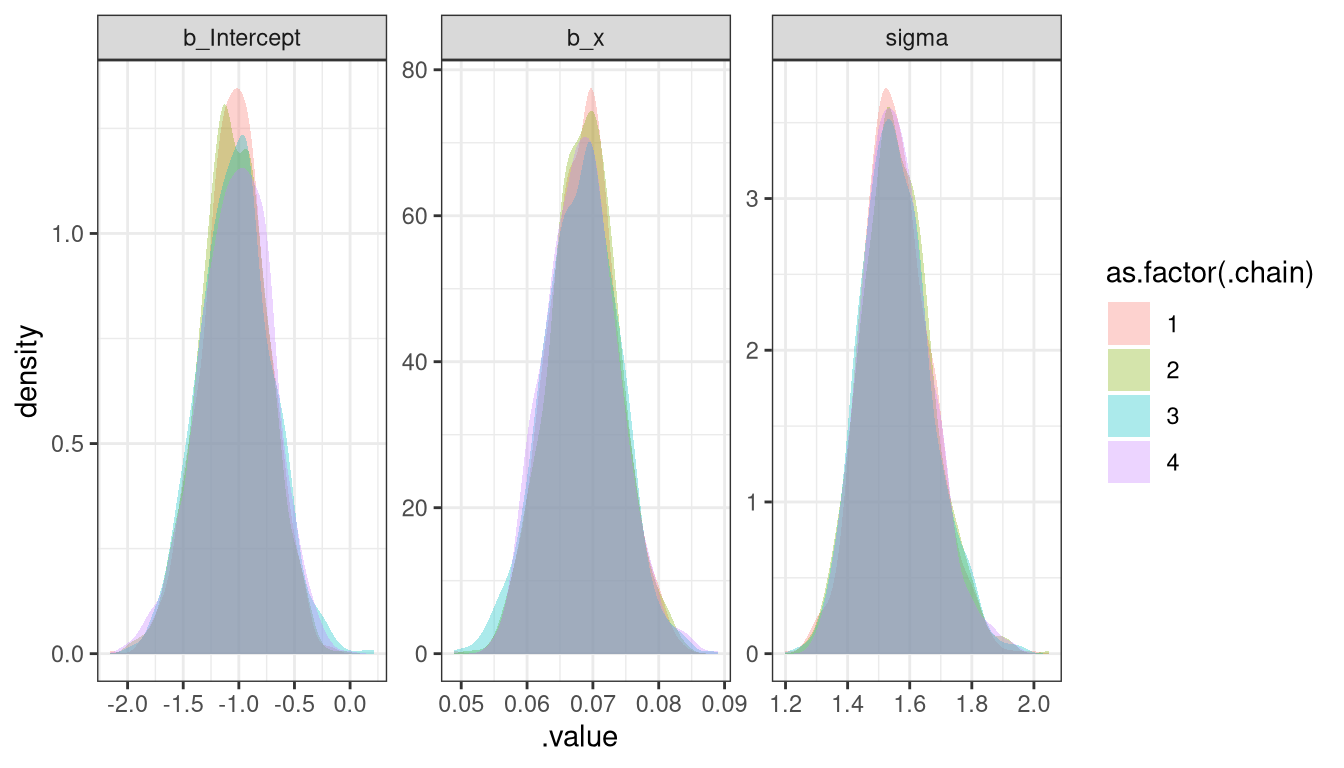
\includegraphics[width=\textwidth]{Lec09_files/figure-beamer/unnamed-chunk-7-1} \end{center}

\end{frame}

\begin{frame}{Differencing - Order 1}
\protect\hypertarget{differencing---order-1}{}

\begin{center}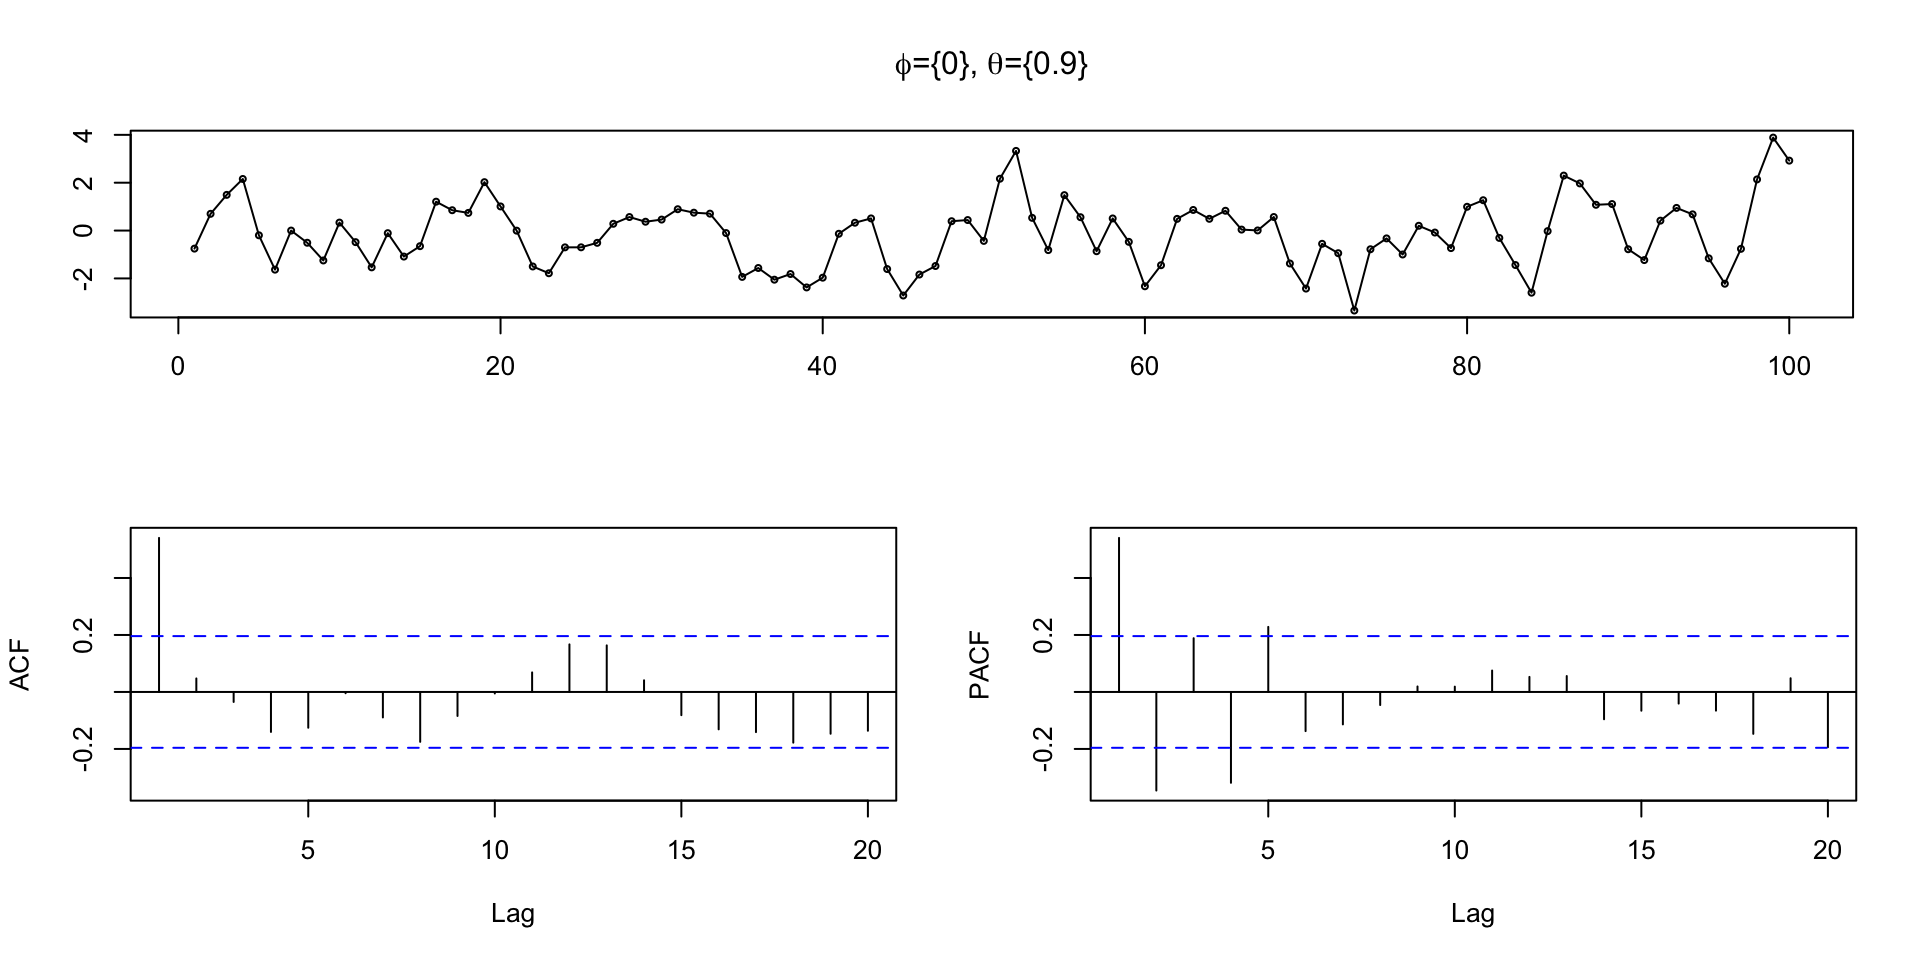
\includegraphics[width=\textwidth]{Lec09_files/figure-beamer/unnamed-chunk-8-1} \end{center}

\end{frame}

\begin{frame}{Differencing - Order 2}
\protect\hypertarget{differencing---order-2}{}

\begin{center}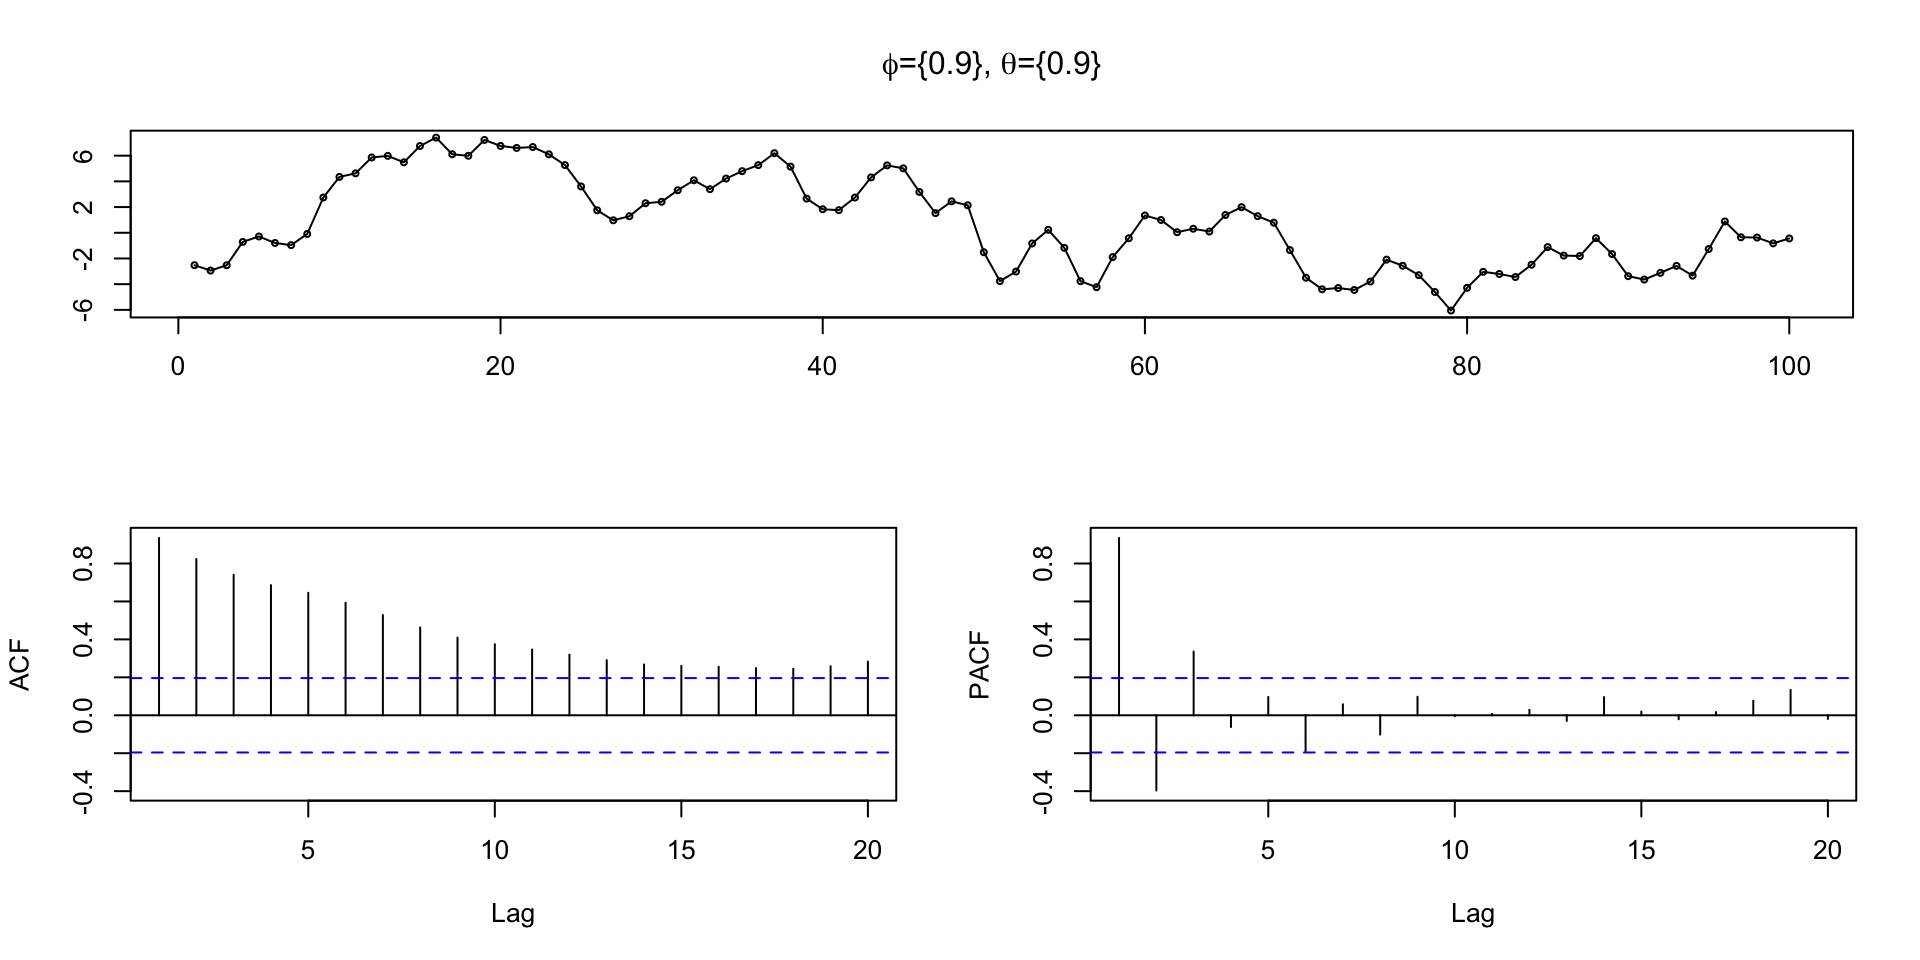
\includegraphics[width=\textwidth]{Lec09_files/figure-beamer/unnamed-chunk-9-1} \end{center}

\end{frame}

\begin{frame}{Differencing - Order 3}
\protect\hypertarget{differencing---order-3}{}

\begin{center}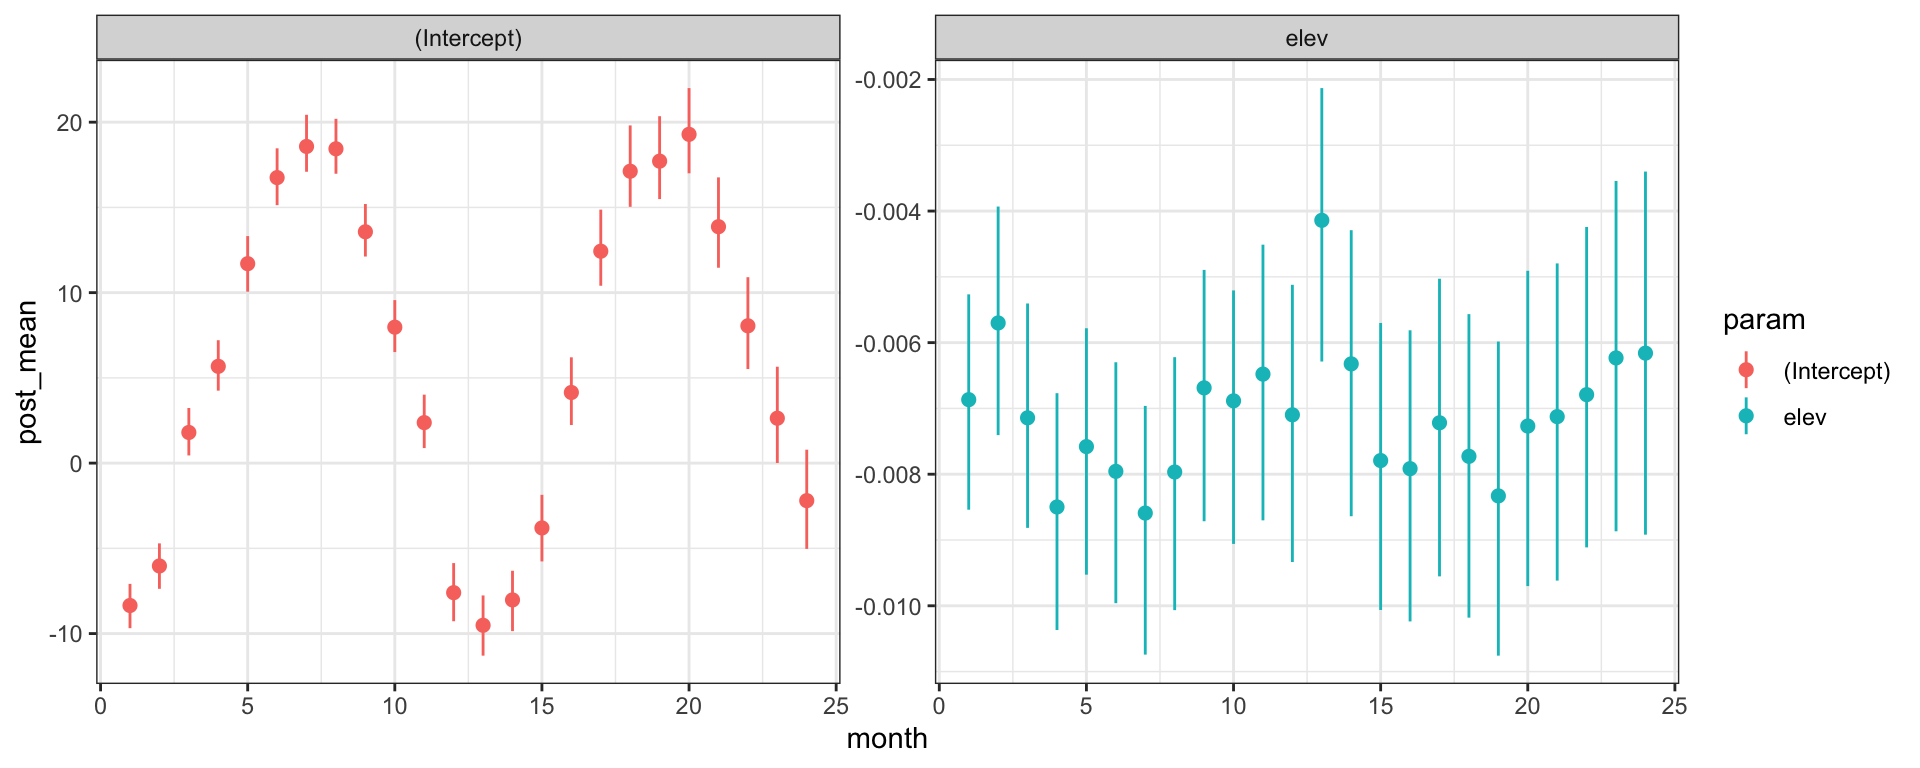
\includegraphics[width=\textwidth]{Lec09_files/figure-beamer/unnamed-chunk-10-1} \end{center}

\end{frame}

\begin{frame}{AR or MA - Time Series 1?}
\protect\hypertarget{ar-or-ma---time-series-1}{}

\begin{center}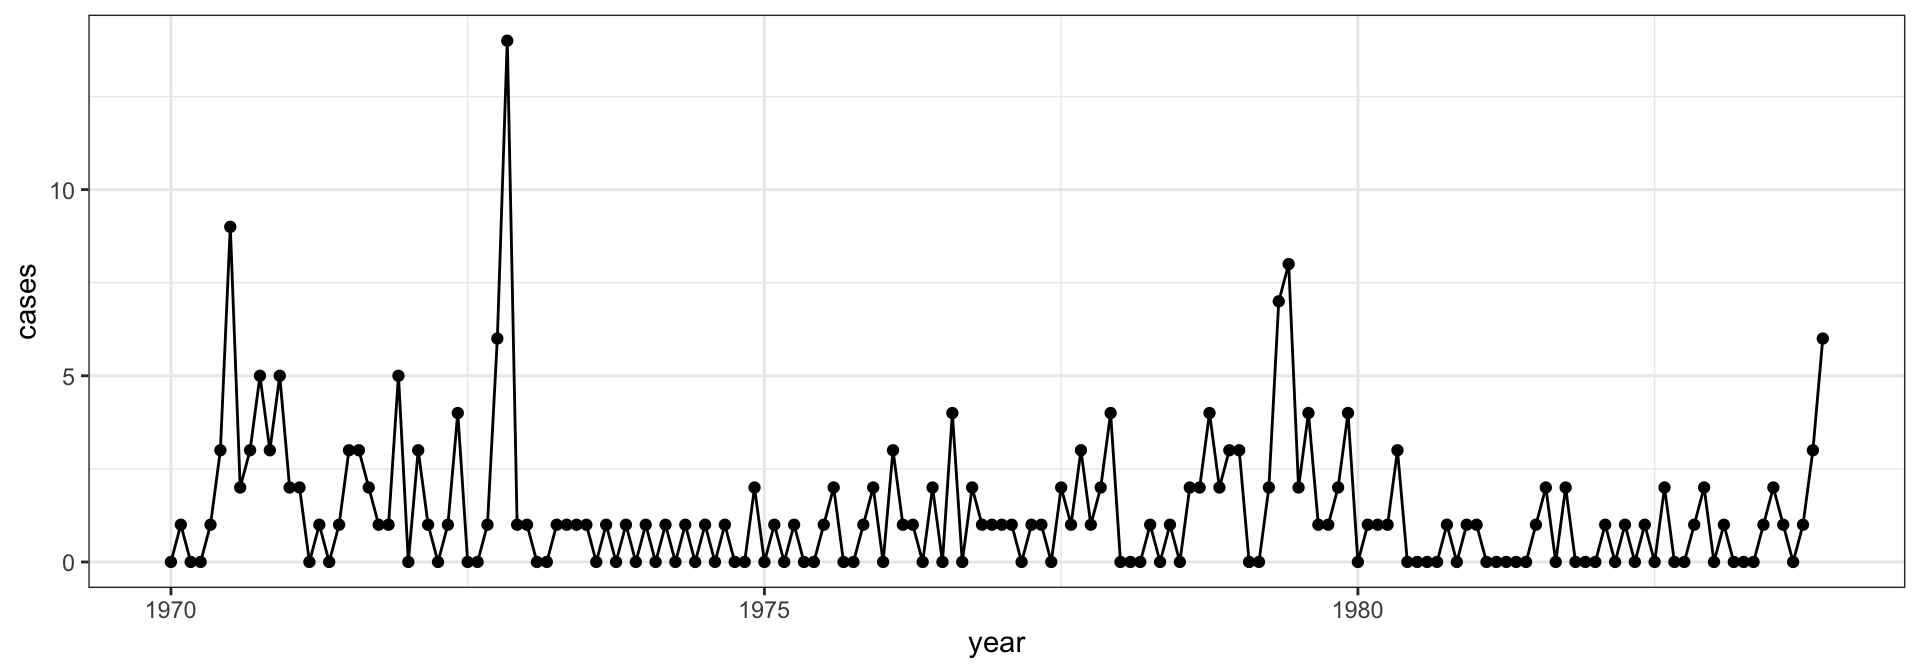
\includegraphics[width=\textwidth]{Lec09_files/figure-beamer/unnamed-chunk-11-1} \end{center}

\end{frame}

\begin{frame}{EDA}
\protect\hypertarget{eda-1}{}

\begin{center}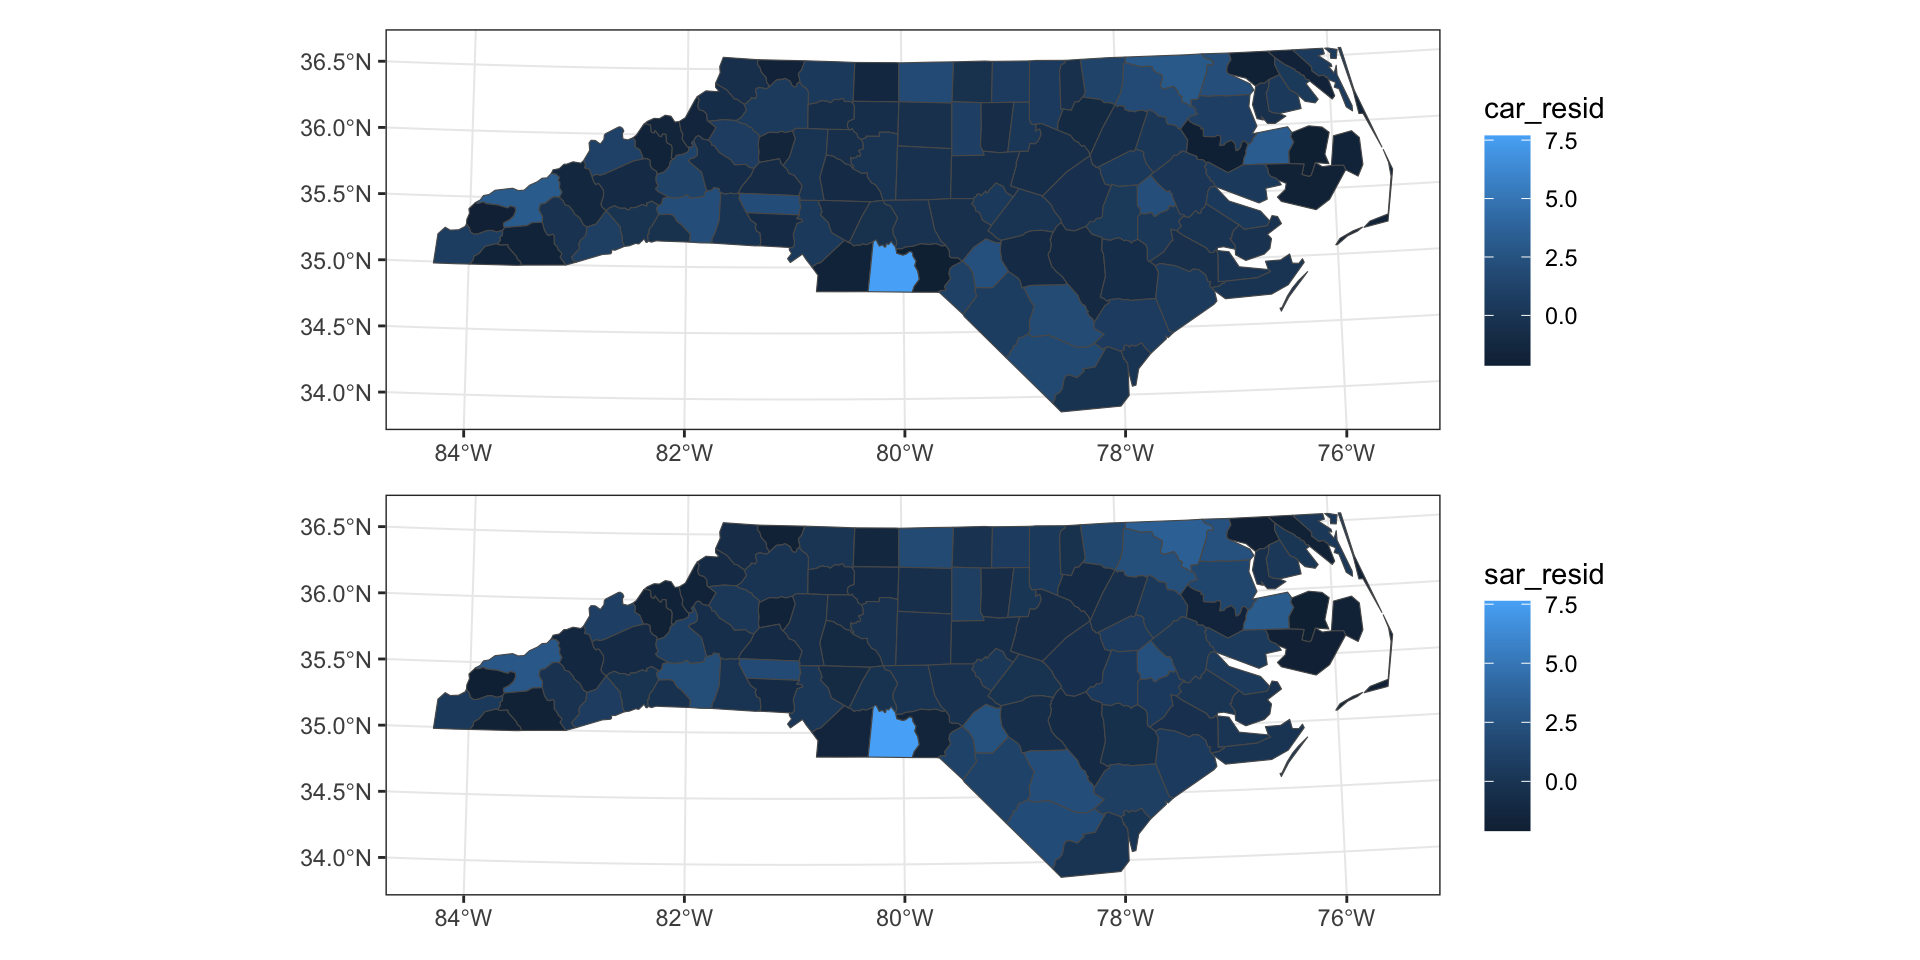
\includegraphics[width=\textwidth]{Lec09_files/figure-beamer/unnamed-chunk-12-1} \end{center}

\end{frame}

\begin{frame}{\texttt{ts1} - Finding \(d\)}
\protect\hypertarget{ts1---finding-d}{}

\begin{center}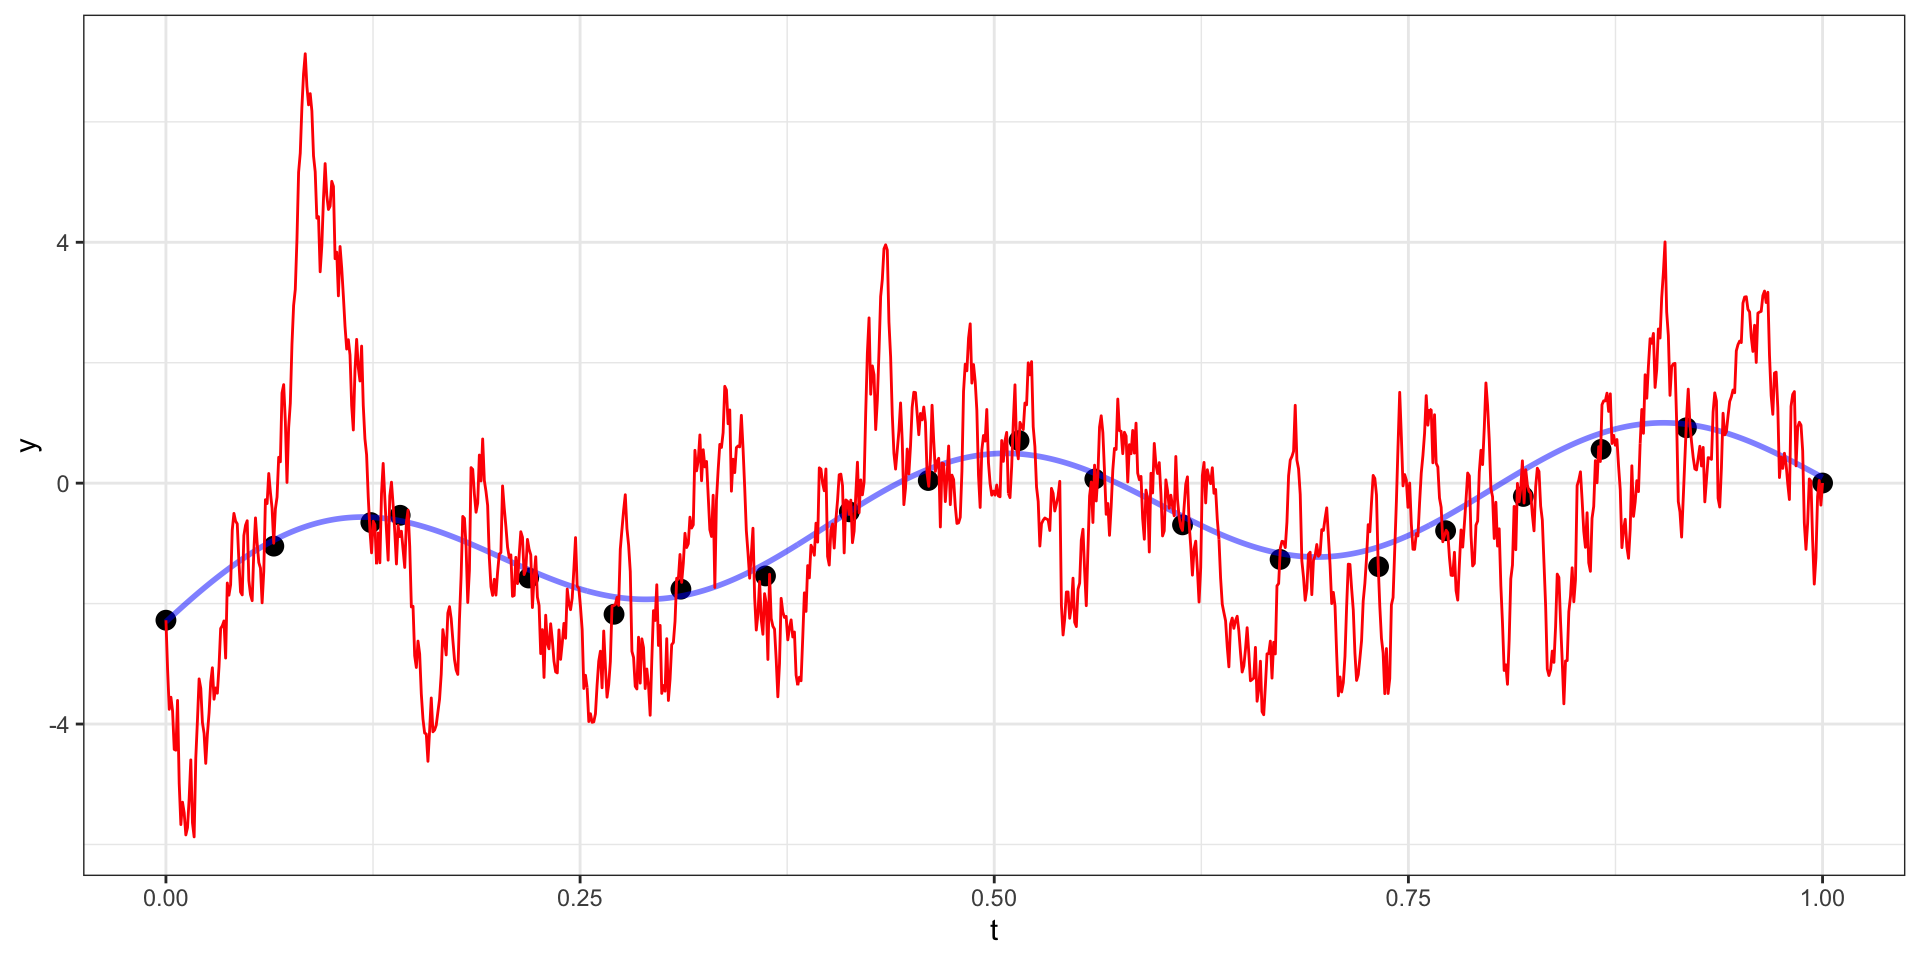
\includegraphics[width=\textwidth]{Lec09_files/figure-beamer/unnamed-chunk-13-1} \end{center}

\end{frame}

\begin{frame}{\texttt{ts2} - Finding \(d\)}
\protect\hypertarget{ts2---finding-d}{}

\begin{center}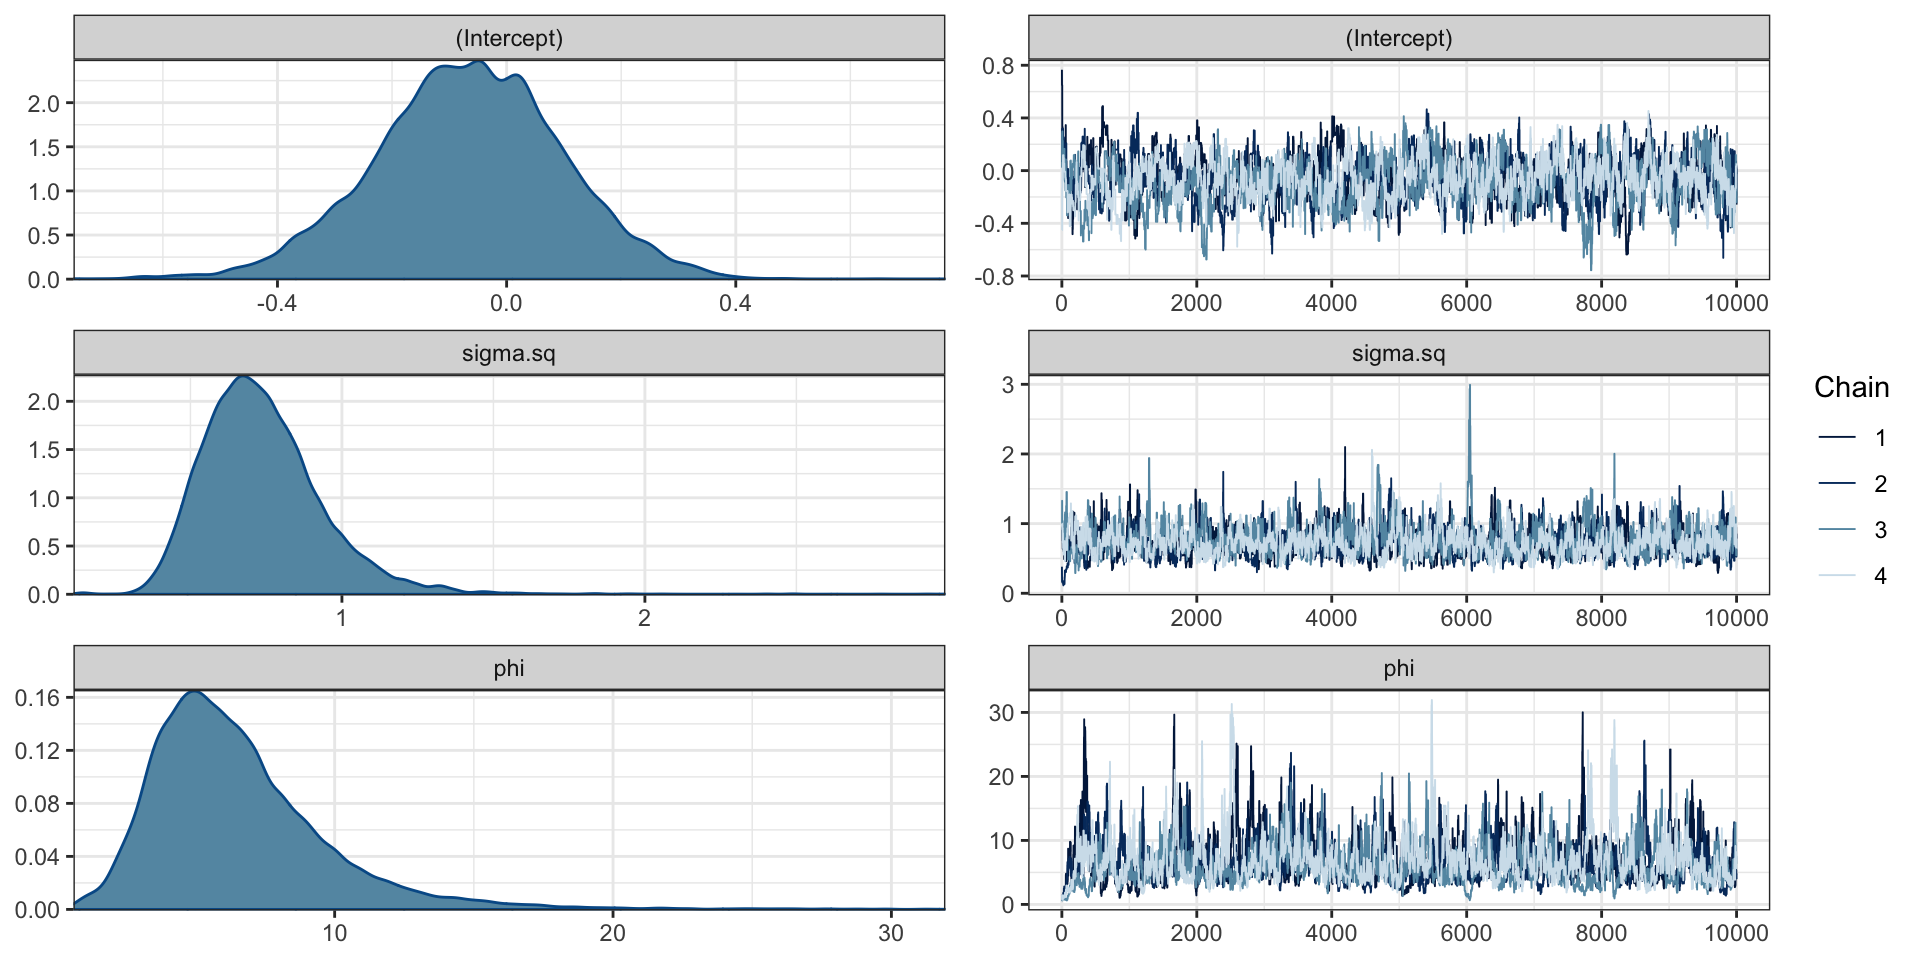
\includegraphics[width=\textwidth]{Lec09_files/figure-beamer/unnamed-chunk-14-1} \end{center}

\end{frame}

\begin{frame}{\texttt{ts1} - Models}
\protect\hypertarget{ts1---models}{}

\begin{longtable}[]{@{}rrrrrr@{}}
\toprule
p & d & q & aic & aicc & bic\tabularnewline
\midrule
\endhead
0 & 1 & 0 & 830.71 & 830.73 & 834.23\tabularnewline
1 & 1 & 0 & 751.57 & 751.62 & 758.61\tabularnewline
2 & 1 & 0 & 745.00 & 745.10 & 755.56\tabularnewline
0 & 1 & 1 & 784.70 & 784.75 & 791.74\tabularnewline
1 & 1 & 1 & 749.63 & 749.73 & 760.20\tabularnewline
2 & 1 & 1 & 739.39 & 739.55 & 753.47\tabularnewline
0 & 1 & 2 & 726.90 & 727.00 & 737.47\tabularnewline
1 & 1 & 2 & 723.19 & 723.35 & 737.27\tabularnewline
2 & 1 & 2 & 725.14 & 725.39 & 742.75\tabularnewline
\bottomrule
\end{longtable}

\end{frame}

\begin{frame}{\texttt{ts2} - Models}
\protect\hypertarget{ts2---models}{}

\begin{longtable}[]{@{}rrrrrr@{}}
\toprule
p & d & q & aic & aicc & bic\tabularnewline
\midrule
\endhead
0 & 1 & 0 & 967.07 & 967.09 & 970.60\tabularnewline
1 & 1 & 0 & 800.69 & 800.74 & 807.74\tabularnewline
2 & 1 & 0 & 756.04 & 756.14 & 766.61\tabularnewline
0 & 1 & 1 & 885.78 & 885.83 & 892.82\tabularnewline
1 & 1 & 1 & 762.34 & 762.43 & 772.90\tabularnewline
2 & 1 & 1 & 756.77 & 756.93 & 770.85\tabularnewline
0 & 1 & 2 & 822.62 & 822.72 & 833.19\tabularnewline
1 & 1 & 2 & 756.88 & 757.05 & 770.97\tabularnewline
2 & 1 & 2 & 758.50 & 758.74 & 776.10\tabularnewline
\bottomrule
\end{longtable}

\end{frame}

\begin{frame}[fragile,t]{\texttt{ts1} - final model}
\protect\hypertarget{ts1---final-model}{}

\scriptoutput

Fitted:

\begin{Shaded}
\begin{Highlighting}[]
\NormalTok{forecast}\OperatorTok{::}\KeywordTok{Arima}\NormalTok{(ts1, }\DataTypeTok{order =} \KeywordTok{c}\NormalTok{(}\DecValTok{0}\NormalTok{,}\DecValTok{1}\NormalTok{,}\DecValTok{2}\NormalTok{))}
\CommentTok{## Series: ts1 }
\CommentTok{## ARIMA(0,1,2) }
\CommentTok{## }
\CommentTok{## Coefficients:}
\CommentTok{##          ma1     ma2}
\CommentTok{##       0.3823  0.5217}
\CommentTok{## s.e.  0.0522  0.0613}
\CommentTok{## }
\CommentTok{## sigma^2 estimated as 1.052:  log likelihood=-360.45}
\CommentTok{## AIC=726.9   AICc=727   BIC=737.47}
\end{Highlighting}
\end{Shaded}

Truth:

\begin{Shaded}
\begin{Highlighting}[]
\NormalTok{ts1 =}\StringTok{ }\KeywordTok{arima.sim}\NormalTok{(}\DataTypeTok{n=}\DecValTok{250}\NormalTok{, }\DataTypeTok{model=}\KeywordTok{list}\NormalTok{(}\DataTypeTok{order=}\KeywordTok{c}\NormalTok{(}\DecValTok{0}\NormalTok{,}\DecValTok{1}\NormalTok{,}\DecValTok{2}\NormalTok{), }\DataTypeTok{ma=}\KeywordTok{c}\NormalTok{(}\FloatTok{0.4}\NormalTok{,}\FloatTok{0.5}\NormalTok{))) }
\end{Highlighting}
\end{Shaded}

\end{frame}

\begin{frame}[fragile,t]{\texttt{ts2} - final model}
\protect\hypertarget{ts2---final-model}{}

\scriptoutput

Fitted:

\begin{Shaded}
\begin{Highlighting}[]
\NormalTok{forecast}\OperatorTok{::}\KeywordTok{Arima}\NormalTok{(ts2, }\DataTypeTok{order =} \KeywordTok{c}\NormalTok{(}\DecValTok{2}\NormalTok{,}\DecValTok{1}\NormalTok{,}\DecValTok{0}\NormalTok{))}
\CommentTok{## Series: ts2 }
\CommentTok{## ARIMA(2,1,0) }
\CommentTok{## }
\CommentTok{## Coefficients:}
\CommentTok{##          ar1     ar2}
\CommentTok{##       0.4148  0.4148}
\CommentTok{## s.e.  0.0573  0.0578}
\CommentTok{## }
\CommentTok{## sigma^2 estimated as 1.181:  log likelihood=-375.02}
\CommentTok{## AIC=756.04   AICc=756.14   BIC=766.61}
\end{Highlighting}
\end{Shaded}

Truth:

\begin{Shaded}
\begin{Highlighting}[]
\NormalTok{ts2 =}\StringTok{ }\KeywordTok{arima.sim}\NormalTok{(}\DataTypeTok{n=}\DecValTok{250}\NormalTok{, }\DataTypeTok{model=}\KeywordTok{list}\NormalTok{(}\DataTypeTok{order=}\KeywordTok{c}\NormalTok{(}\DecValTok{2}\NormalTok{,}\DecValTok{1}\NormalTok{,}\DecValTok{0}\NormalTok{), }\DataTypeTok{ar=}\KeywordTok{c}\NormalTok{(}\FloatTok{0.4}\NormalTok{,}\FloatTok{0.5}\NormalTok{))) }
\end{Highlighting}
\end{Shaded}

\end{frame}

\begin{frame}{Residuals}
\protect\hypertarget{residuals}{}

\begin{center}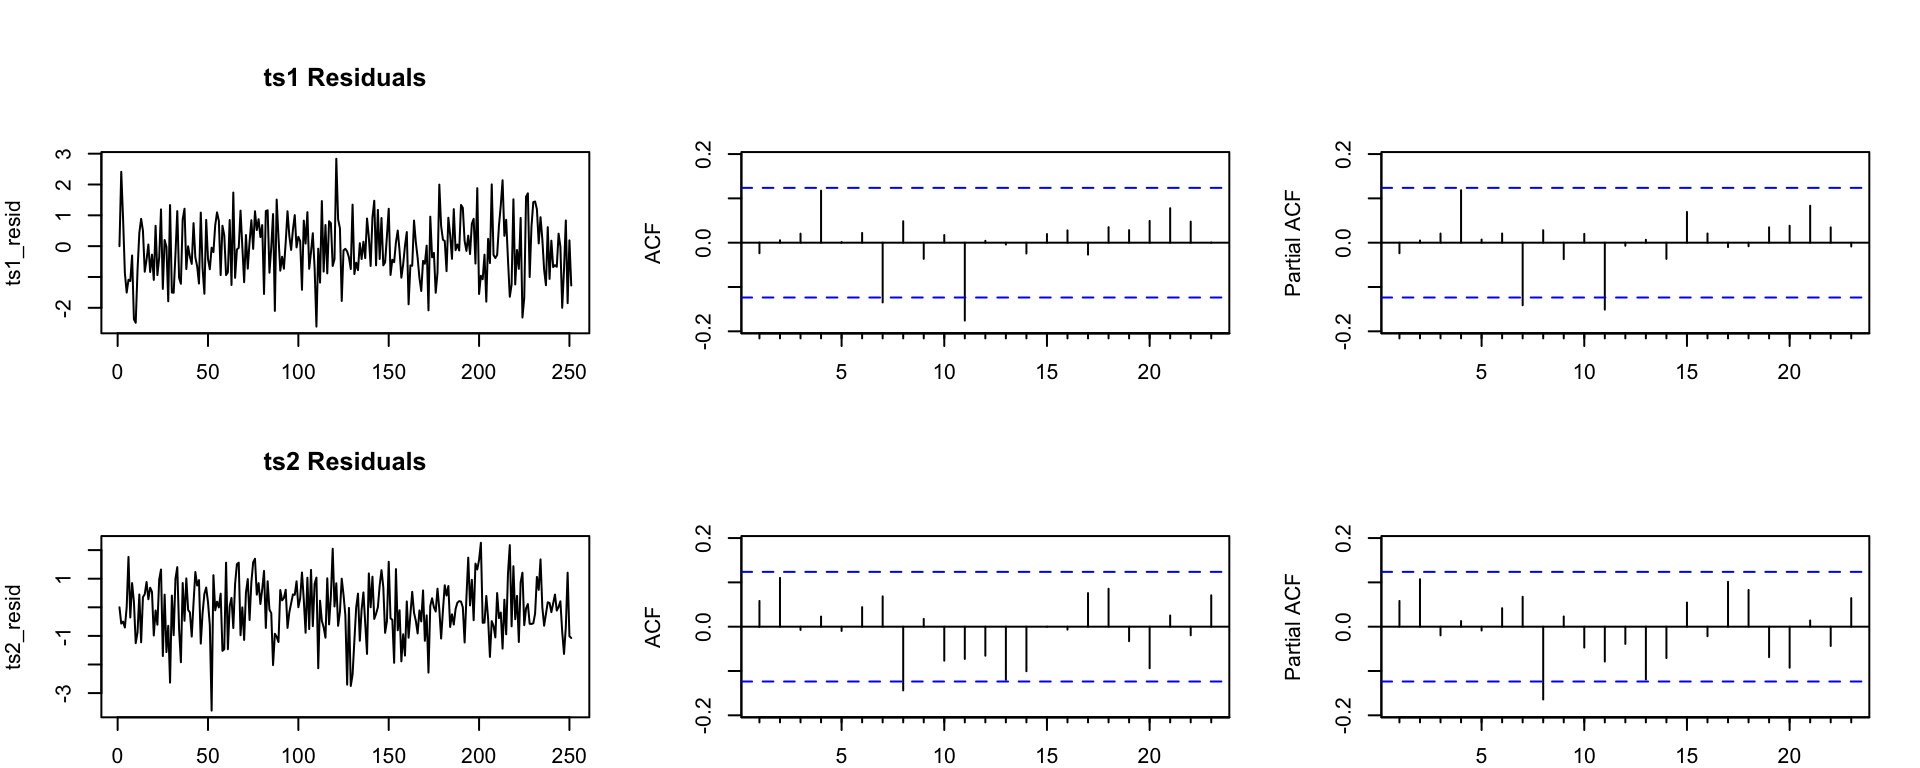
\includegraphics[width=\textwidth]{Lec09_files/figure-beamer/unnamed-chunk-21-1} \end{center}

\end{frame}

\begin{frame}[fragile]{Automatic model selection}
\protect\hypertarget{automatic-model-selection}{}

\scriptoutput

\texttt{ts1}:

\begin{Shaded}
\begin{Highlighting}[]
\NormalTok{forecast}\OperatorTok{::}\KeywordTok{auto.arima}\NormalTok{(ts1)}
\CommentTok{## Series: ts1 }
\CommentTok{## ARIMA(1,1,2) }
\CommentTok{## }
\CommentTok{## Coefficients:}
\CommentTok{##          ar1     ma1     ma2}
\CommentTok{##       0.2804  0.1838  0.4512}
\CommentTok{## s.e.  0.1199  0.1092  0.0736}
\CommentTok{## }
\CommentTok{## sigma^2 estimated as 1.033:  log likelihood=-357.59}
\CommentTok{## AIC=723.19   AICc=723.35   BIC=737.27}
\end{Highlighting}
\end{Shaded}

\texttt{ts2}:

\begin{Shaded}
\begin{Highlighting}[]
\NormalTok{forecast}\OperatorTok{::}\KeywordTok{auto.arima}\NormalTok{(ts2)}
\CommentTok{## Series: ts2 }
\CommentTok{## ARIMA(1,2,1) }
\CommentTok{## }
\CommentTok{## Coefficients:}
\CommentTok{##           ar1      ma1}
\CommentTok{##       -0.3052  -0.2661}
\CommentTok{## s.e.   0.1184   0.1217}
\CommentTok{## }
\CommentTok{## sigma^2 estimated as 1.227:  log likelihood=-377.92}
\CommentTok{## AIC=761.84   AICc=761.94   BIC=772.4}
\end{Highlighting}
\end{Shaded}

\end{frame}

\hypertarget{electrical-equipment-sales}{%
\section{Electrical Equipment Sales}\label{electrical-equipment-sales}}

\begin{frame}{Data}
\protect\hypertarget{data}{}

\begin{center}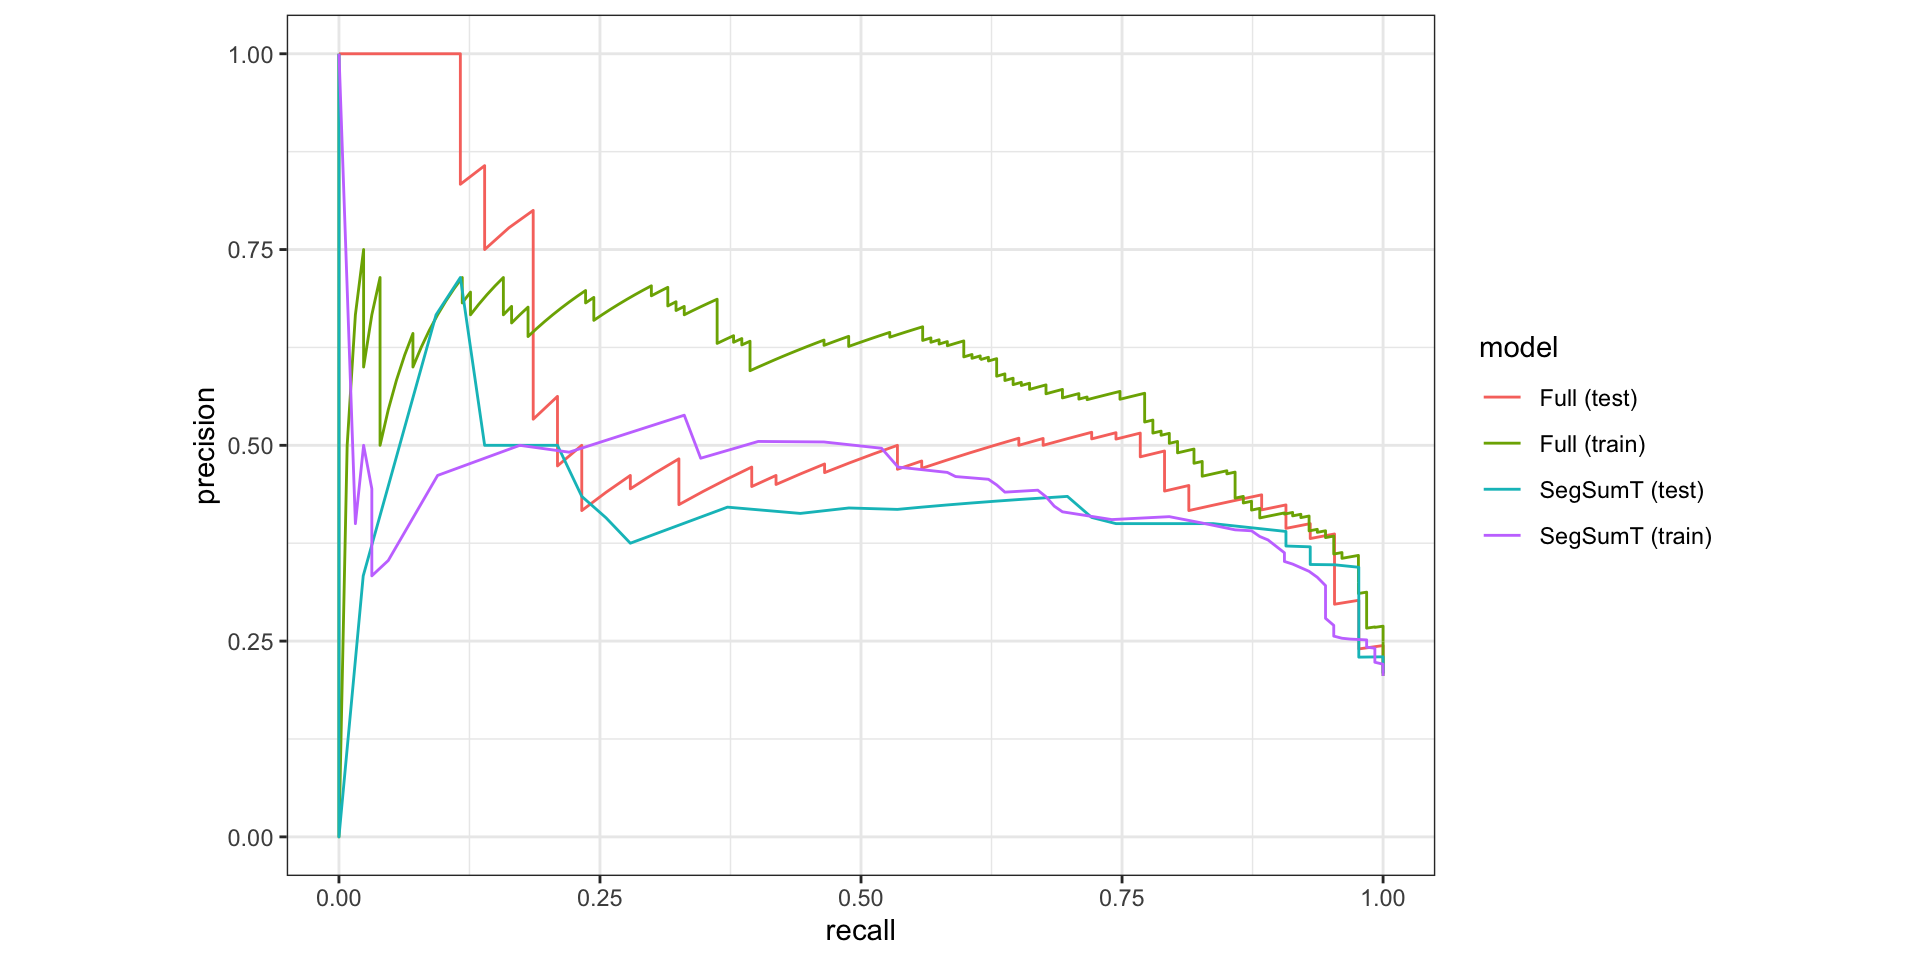
\includegraphics[width=\textwidth]{Lec09_files/figure-beamer/unnamed-chunk-24-1} \end{center}

\end{frame}

\begin{frame}{1st order differencing}
\protect\hypertarget{st-order-differencing}{}

\begin{center}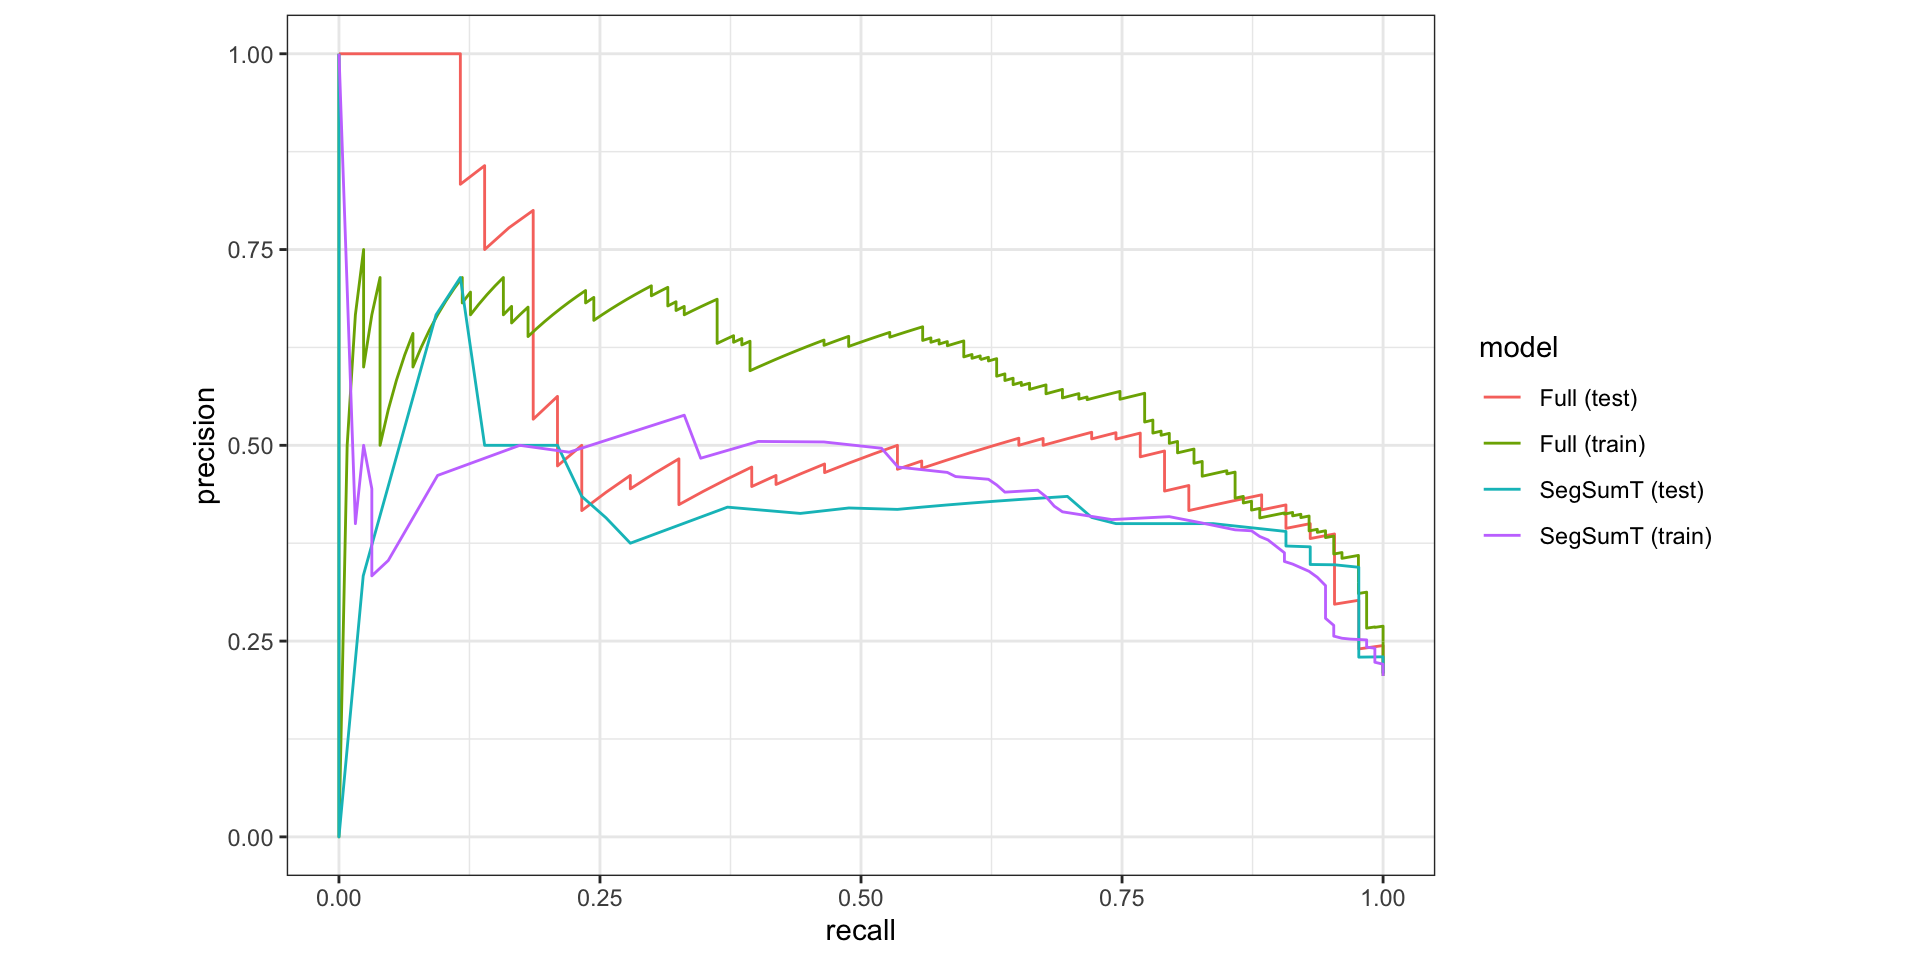
\includegraphics[width=\textwidth]{Lec09_files/figure-beamer/unnamed-chunk-25-1} \end{center}

\end{frame}

\begin{frame}{2nd order differencing}
\protect\hypertarget{nd-order-differencing}{}

\begin{center}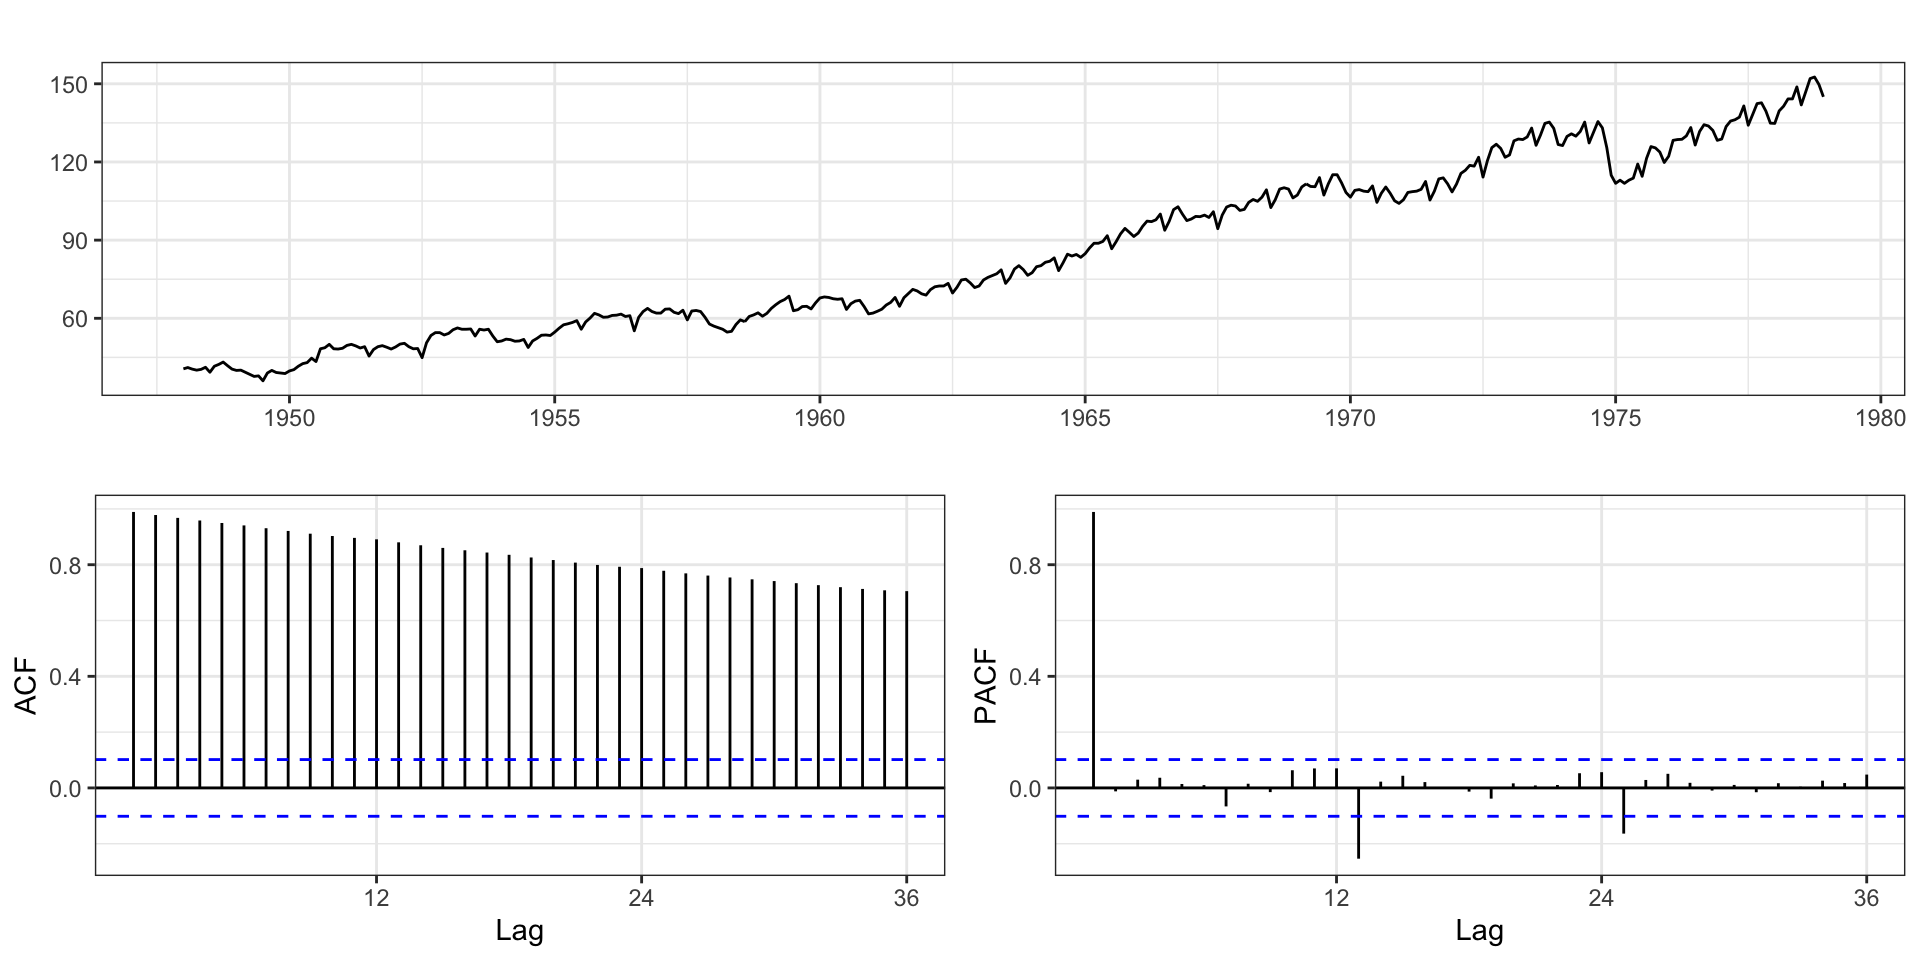
\includegraphics[width=\textwidth]{Lec09_files/figure-beamer/unnamed-chunk-26-1} \end{center}

\end{frame}

\begin{frame}[fragile,t]{Model}
\protect\hypertarget{model}{}

\begin{Shaded}
\begin{Highlighting}[]
\NormalTok{forecast}\OperatorTok{::}\KeywordTok{Arima}\NormalTok{(elec_sales, }\DataTypeTok{order =} \KeywordTok{c}\NormalTok{(}\DecValTok{3}\NormalTok{,}\DecValTok{1}\NormalTok{,}\DecValTok{0}\NormalTok{))}
\CommentTok{## Series: elec_sales }
\CommentTok{## ARIMA(3,1,0) }
\CommentTok{## }
\CommentTok{## Coefficients:}
\CommentTok{##           ar1      ar2     ar3}
\CommentTok{##       -0.3488  -0.0386  0.3139}
\CommentTok{## s.e.   0.0690   0.0736  0.0694}
\CommentTok{## }
\CommentTok{## sigma^2 estimated as 9.853:  log likelihood=-485.67}
\CommentTok{## AIC=979.33   AICc=979.55   BIC=992.32}
\end{Highlighting}
\end{Shaded}

\end{frame}

\begin{frame}[fragile]{Residuals}
\protect\hypertarget{residuals-1}{}

\begin{Shaded}
\begin{Highlighting}[]
\NormalTok{forecast}\OperatorTok{::}\KeywordTok{Arima}\NormalTok{(elec_sales, }\DataTypeTok{order =} \KeywordTok{c}\NormalTok{(}\DecValTok{3}\NormalTok{,}\DecValTok{1}\NormalTok{,}\DecValTok{0}\NormalTok{)) }\OperatorTok\StringTok{ }\KeywordTok{residuals}\NormalTok{() }\OperatorTok\StringTok{ }
\StringTok{  }\NormalTok{forecast}\OperatorTok{::}\KeywordTok{tsdisplay}\NormalTok{(}\DataTypeTok{points=}\OtherTok{FALSE}\NormalTok{)}
\end{Highlighting}
\end{Shaded}

\begin{center}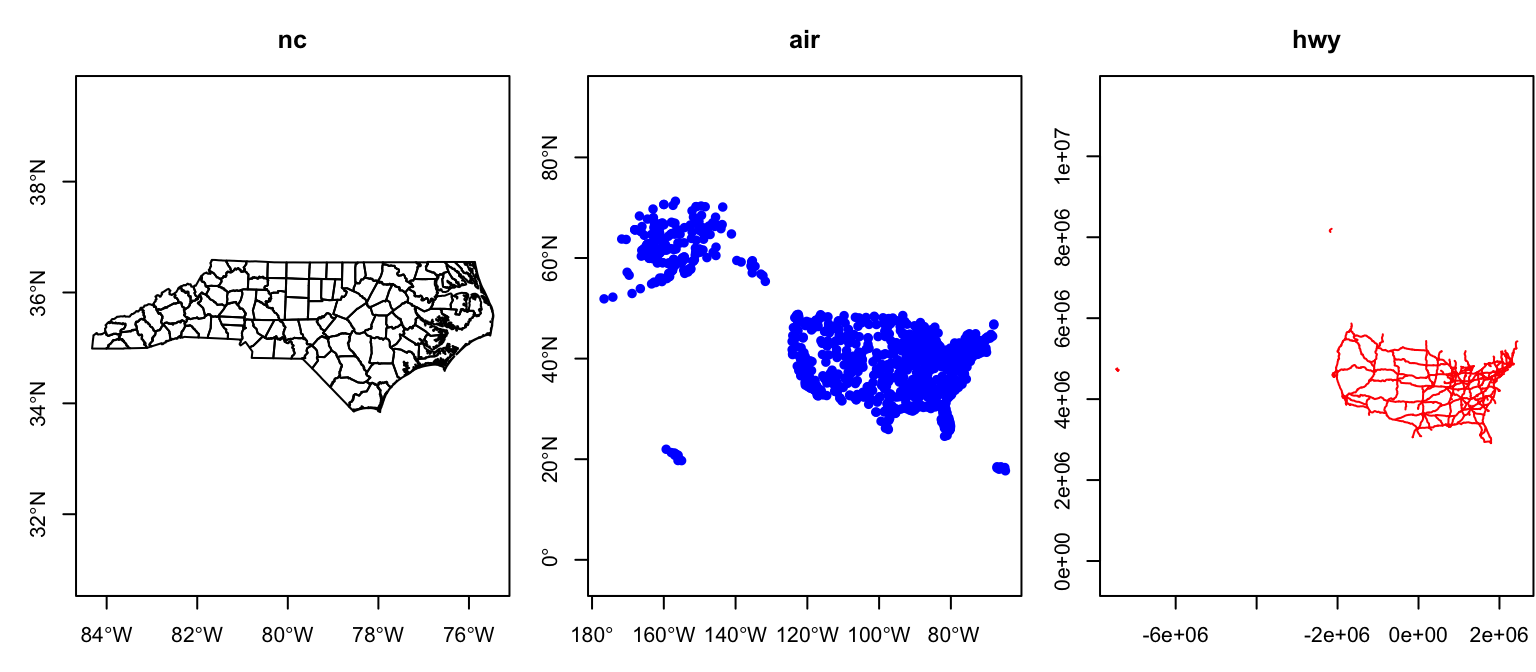
\includegraphics[width=\textwidth]{Lec09_files/figure-beamer/unnamed-chunk-29-1} \end{center}

\end{frame}

\begin{frame}[fragile]{Model Comparison}
\protect\hypertarget{model-comparison}{}

\scriptoutput

Model choices:

\begin{Shaded}
\begin{Highlighting}[]
\NormalTok{forecast}\OperatorTok{::}\KeywordTok{Arima}\NormalTok{(elec_sales, }\DataTypeTok{order =} \KeywordTok{c}\NormalTok{(}\DecValTok{3}\NormalTok{,}\DecValTok{1}\NormalTok{,}\DecValTok{0}\NormalTok{))}\OperatorTok{$}\NormalTok{aicc}
\CommentTok{## [1] 979.5477}

\NormalTok{forecast}\OperatorTok{::}\KeywordTok{Arima}\NormalTok{(elec_sales, }\DataTypeTok{order =} \KeywordTok{c}\NormalTok{(}\DecValTok{3}\NormalTok{,}\DecValTok{1}\NormalTok{,}\DecValTok{1}\NormalTok{))}\OperatorTok{$}\NormalTok{aicc}
\CommentTok{## [1] 978.4925}

\NormalTok{forecast}\OperatorTok{::}\KeywordTok{Arima}\NormalTok{(elec_sales, }\DataTypeTok{order =} \KeywordTok{c}\NormalTok{(}\DecValTok{4}\NormalTok{,}\DecValTok{1}\NormalTok{,}\DecValTok{0}\NormalTok{))}\OperatorTok{$}\NormalTok{aicc}
\CommentTok{## [1] 979.2309}

\NormalTok{forecast}\OperatorTok{::}\KeywordTok{Arima}\NormalTok{(elec_sales, }\DataTypeTok{order =} \KeywordTok{c}\NormalTok{(}\DecValTok{2}\NormalTok{,}\DecValTok{1}\NormalTok{,}\DecValTok{0}\NormalTok{))}\OperatorTok{$}\NormalTok{aicc}
\CommentTok{## [1] 996.8085}
\end{Highlighting}
\end{Shaded}

Automatic selection:

\begin{Shaded}
\begin{Highlighting}[]
\NormalTok{forecast}\OperatorTok{::}\KeywordTok{auto.arima}\NormalTok{(elec_sales)}
\CommentTok{## Series: elec_sales }
\CommentTok{## ARIMA(3,1,1) }
\CommentTok{## }
\CommentTok{## Coefficients:}
\CommentTok{##          ar1     ar2     ar3      ma1}
\CommentTok{##       0.0519  0.1191  0.3730  -0.4542}
\CommentTok{## s.e.  0.1840  0.0888  0.0679   0.1993}
\CommentTok{## }
\CommentTok{## sigma^2 estimated as 9.737:  log likelihood=-484.08}
\CommentTok{## AIC=978.17   AICc=978.49   BIC=994.4}
\end{Highlighting}
\end{Shaded}

\end{frame}

\begin{frame}{Model fit}
\protect\hypertarget{model-fit}{}

\begin{center}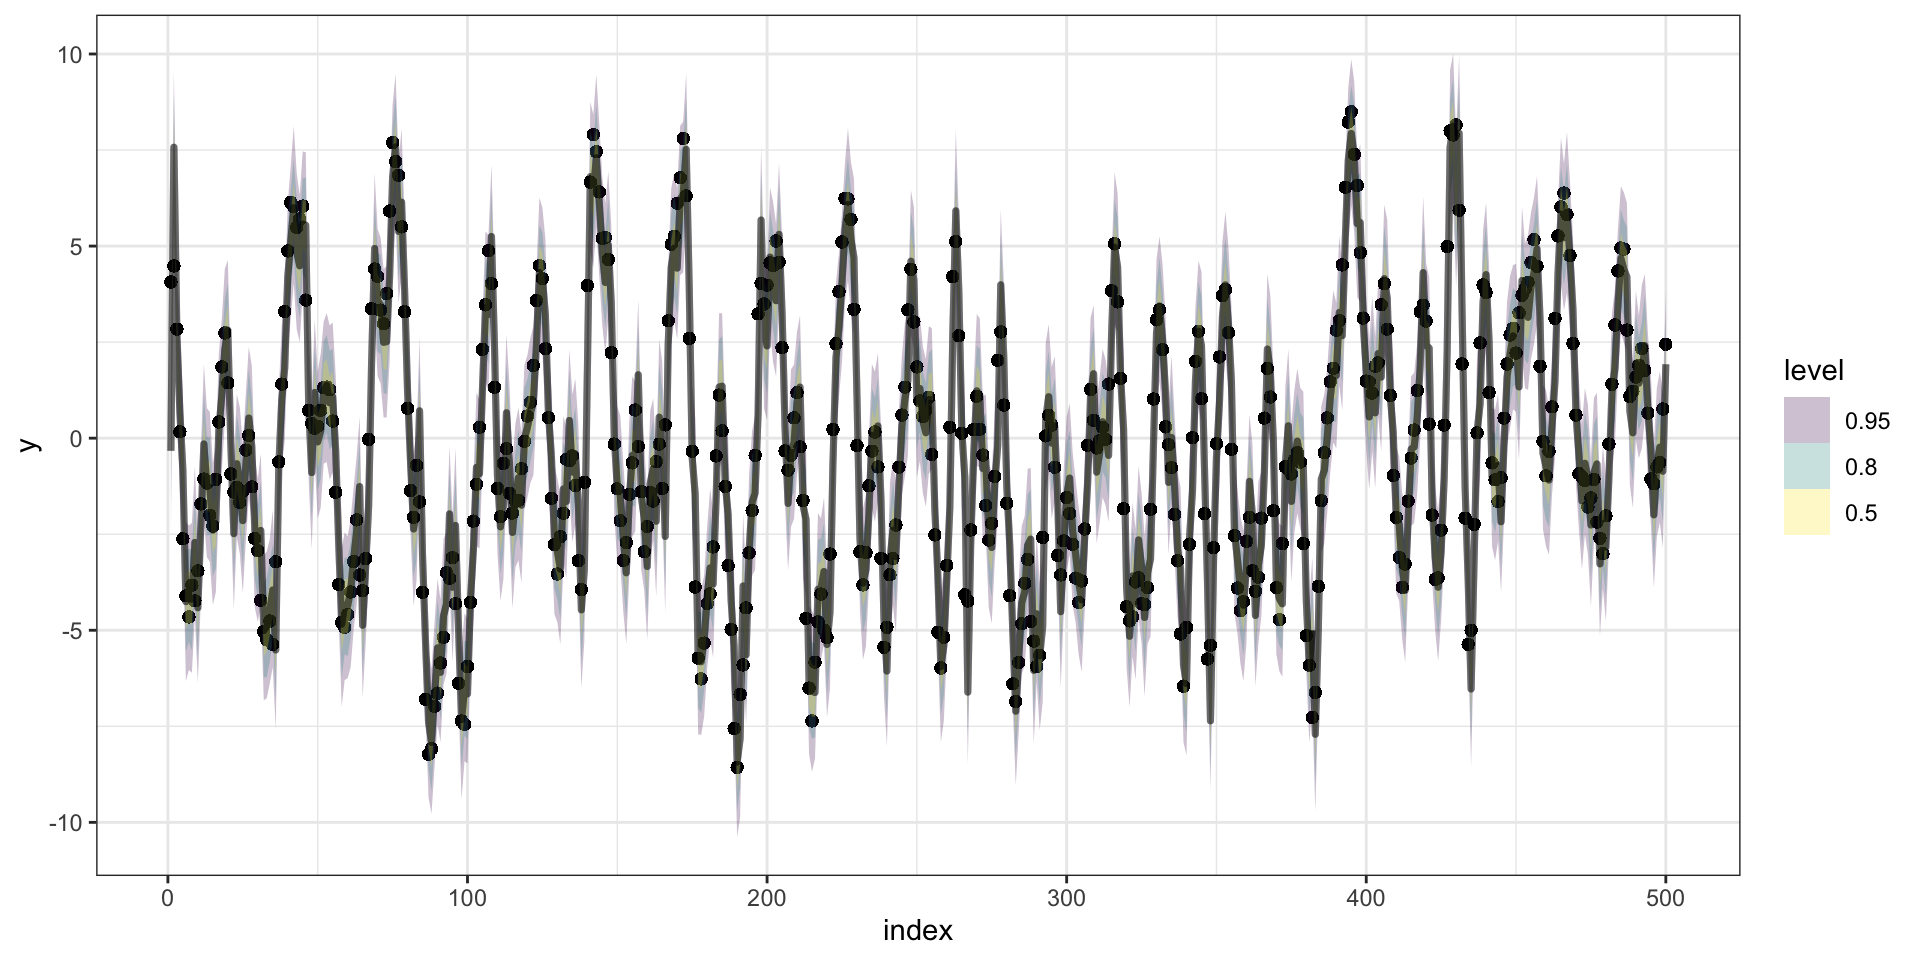
\includegraphics[width=\textwidth]{Lec09_files/figure-beamer/unnamed-chunk-32-1} \end{center}

\end{frame}

\begin{frame}[fragile]{Model forecast}
\protect\hypertarget{model-forecast}{}

\begin{Shaded}
\begin{Highlighting}[]
\NormalTok{forecast}\OperatorTok{::}\KeywordTok{Arima}\NormalTok{(elec_sales, }\DataTypeTok{order =} \KeywordTok{c}\NormalTok{(}\DecValTok{3}\NormalTok{,}\DecValTok{1}\NormalTok{,}\DecValTok{0}\NormalTok{)) }\OperatorTok\StringTok{ }
\StringTok{  }\NormalTok{forecast}\OperatorTok{::}\KeywordTok{forecast}\NormalTok{() }\OperatorTok\StringTok{ }\KeywordTok{autoplot}\NormalTok{()}
\end{Highlighting}
\end{Shaded}

\begin{center}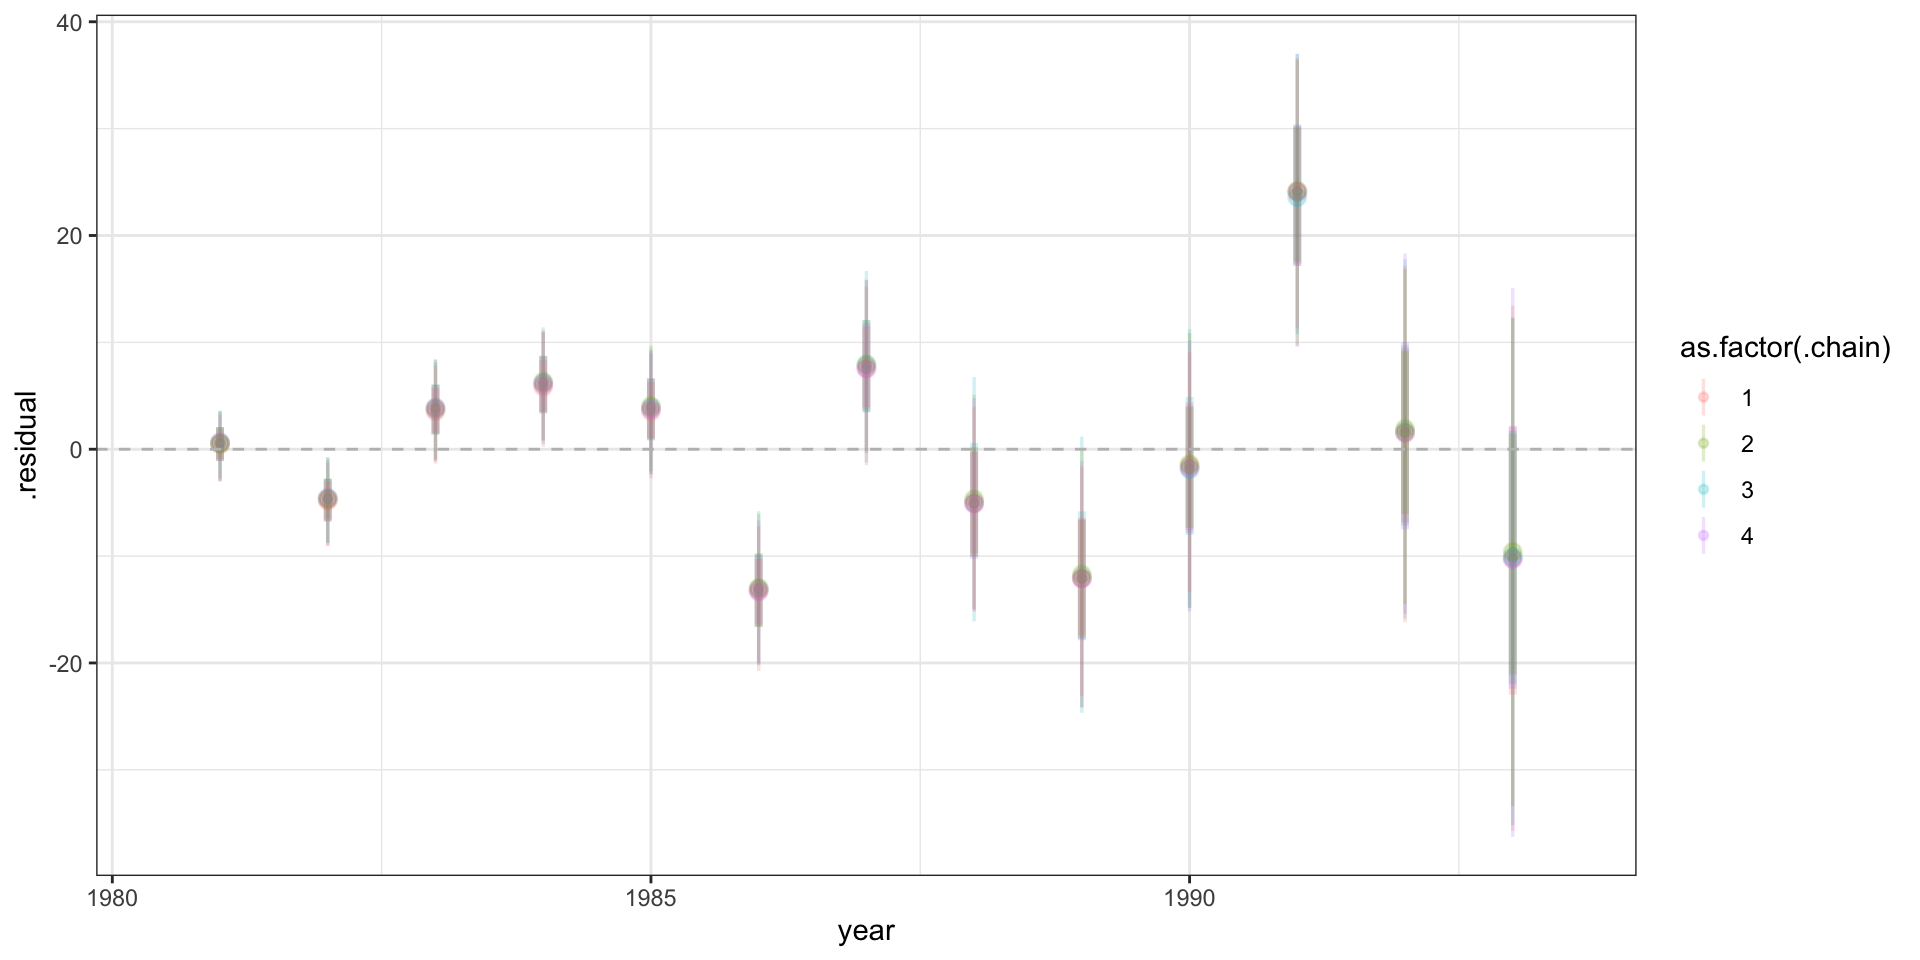
\includegraphics[width=\textwidth]{Lec09_files/figure-beamer/unnamed-chunk-33-1} \end{center}

\end{frame}

\begin{frame}[fragile]{Model forecast - Zoom}
\protect\hypertarget{model-forecast---zoom}{}

\begin{Shaded}
\begin{Highlighting}[]
\NormalTok{forecast}\OperatorTok{::}\KeywordTok{Arima}\NormalTok{(elec_sales, }\DataTypeTok{order =} \KeywordTok{c}\NormalTok{(}\DecValTok{3}\NormalTok{,}\DecValTok{1}\NormalTok{,}\DecValTok{0}\NormalTok{)) }\OperatorTok\StringTok{ }
\StringTok{  }\NormalTok{forecast}\OperatorTok{::}\KeywordTok{forecast}\NormalTok{() }\OperatorTok\StringTok{ }\KeywordTok{autoplot}\NormalTok{() }\OperatorTok{+}\StringTok{ }\KeywordTok{xlim}\NormalTok{(}\DecValTok{2009}\NormalTok{,}\DecValTok{2014}\NormalTok{)}
\end{Highlighting}
\end{Shaded}

\begin{center}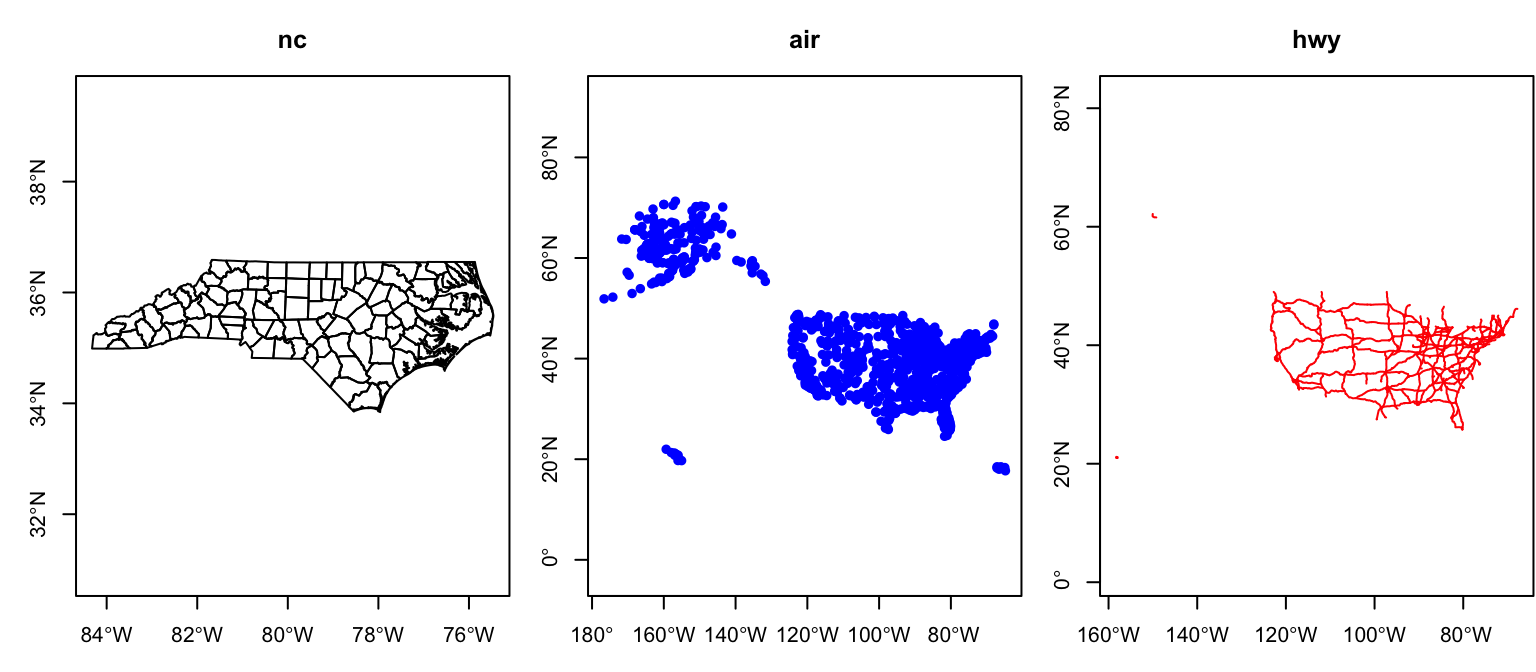
\includegraphics[width=\textwidth]{Lec09_files/figure-beamer/unnamed-chunk-34-1} \end{center}

\end{frame}

\begin{frame}[t]{General Guidance}
\protect\hypertarget{general-guidance}{}

\begin{enumerate}
\item
  Positive autocorrelations out to a large number of lags usually
  indicates a need for differencing
\item
  Slightly too much or slightly too little differencing can be corrected
  by adding AR or MA terms respectively.
\item
  A model with no differencing usually includes a constant term, a model
  with two or more orders (rare) differencing usually does not include a
  constant term.
\item
  After differencing, if the PACF has a sharp cutoff then consider
  adding AR terms to the model.
\item
  After differencing, if the ACF has a sharp cutoff then consider adding
  an MA term to the model.
\item
  It is possible for an AR term and an MA term to cancel each other's
  effects, so try models with one fewer AR term and one fewer MA term.
\end{enumerate}

\scriptsize{Based on rules from \url{https://people.duke.edu/~rnau/411arim2.htm} and \url{https://people.duke.edu/~rnau/411arim3.htm}}

\end{frame}

\end{document}
